\documentclass[14pt,a4paper]{article}
\usepackage{mathtools}
\usepackage{amsmath}
\usepackage{bigints}
\usepackage{mathrsfs}
\usepackage{setspace}
\usepackage{amsfonts}
\usepackage{geometry}
\geometry{a4paper, total = {210mm,297mm},left=22mm, right=20mm,top=20mm,bottom=20mm}
\usepackage{xcolor}
\usepackage{mcode}
\usepackage{listings}
\lstset{basicstyle = \fontsize{11}{12} \selectfont\ttfamily}
\usepackage{subfig}
\usepackage{graphicx}


%Begin document - Vibration Mechanic Systems - Final Project

\begin{document}
\label{cover}
\begin{center}
	\vspace*{3cm}
	\large{\textbf{ME 5514 VIBRATION MECHANICS SYSTEMS \\ Final Project}}
	\vfill
	\textbf{Luan Cong Doan} \\ luandoan@vt.edu
	%\vfill
%	Department of Mechanical Engineering \\ Virginia Polytechnic Institute and State University
	\vfill
	\today
\end{center}
\pagebreak

\label{Answer Sheet}
\label{Vibration Mechanics _ Final Project}
\doublespacing
\textbf{Problem 1.} Consider the $\mathrm{d}x$ element of the given cantilever beam we have: $V$ and $M$ are the shear force and bending moments respectively.\\
- Summing the force in $Y$-direction for the $\mathrm{d}m$ elements:\\
\hspace*{5cm} $\mathrm{d}m\bar{Y} = \sum F_y \Leftrightarrow \rho A\dfrac{\partial^2Y}{\partial t^2} = -\dfrac{\partial V}{\partial X} $\\
with: $\rho$ is the density (mass/volume): $\rho = 2.7$  $g/cm^3$ \\
\hspace*{0.8cm} $A$ is the cross-sectional area: $A = 0.32*2.45 = 0.784$ $cm^2$ \\
The bending moment $M$ is defined by: $M = EI\dfrac{\partial^2Y}{\partial X^2}$ with $I$ is moment inertial of cross-sectional\\
\hspace*{1cm}	$I = \dfrac{bh^3}{12} = \dfrac{2.45*10^{-2}*(3.2*10^{-3})^3}{12} = 6.69\times 10^{-11}$ $m^4$\\
The shear force $V$ is calculated from $M$: $V = \dfrac{\partial M}{\partial X} $\\
Because $EI$ is constant, we come up with: $\dfrac{\partial^2Y}{\partial t^2} + \dfrac{EI}{\rho A}\dfrac{\partial^4Y}{\partial X^4} = 0$ \hspace{2cm} (1)\\
Assume the vibration solution is: $Y(X,t) = \bar{Y}(X)\sin\omega t$\\
(1) become: $\dfrac{\mathrm{d}^4\bar{Y}}{\mathrm{d}X^4} - \beta^4\bar{Y} = 0$ \hspace{2cm} with $ \beta^4 = \dfrac{\rho A\omega^2}{EI}$\\
Solution: $\bar{Y}(X) = a\cosh \beta X + b\sinh \beta X + c\cos \beta X + d\sin \beta X $ \hspace{2cm} (2)
\begin{enumerate}
	\item Assume the tip mas can be modeled as a point mass $\Rightarrow$ the boundary conditions are:\\
	- End displacement (on left): $Y(0,t) = 0 \Rightarrow \bar{Y}(0) = 0 \Leftrightarrow \bar{Y}(0) = a + c = 0$ \hspace{1cm} (3)\\
	- End slope (on left): $Y'(0,t) = 0 \Rightarrow \bar{Y}'(0) = 0$\\
	with $ \bar{Y}'(X,t) = \beta a \sinh \beta X + \beta b \cosh \beta X - \beta c \sin \beta X + \beta d \cos \beta X $\\
	$\Rightarrow \bar{Y}'(0,t) = \beta b + \beta d = 0 \Leftrightarrow b + d = 0$ \hspace{6.5cm} (4) \\
	- End moment (on right): $ M(L,t) = EI\dfrac{\partial^2Y}{\partial X^2} (L,t) = 0 \Leftrightarrow \bar{Y}''(L,t) = 0$\\
	with $ \bar{Y}''(X,t) = \beta^2 a \cosh \beta X + \beta^2 b \sinh \beta X - \beta^2 c \cos \beta X - \beta^2 d \sin \beta X $\\
	$\Rightarrow \bar{Y}''(L,t) = \beta^2 \left(a \cosh \beta L + b \sinh \beta L - c \cos \beta L - d \sin \beta L \right) = 0 $\\
	\hspace*{1.6cm} $\Leftrightarrow a \cosh \beta L + b \sinh \beta L - c \cos \beta L - d \sin \beta L = 0 $ \hspace{1cm} (because $\beta \neq 0$) \\
	\hspace*{1.6cm} $ \Leftrightarrow \dfrac{a}{b} = -\dfrac{ \sinh\beta L + \sin \beta L}{\cosh \beta L + \cos \beta L} $ \hspace{6.5cm} (5)\\ 
	- Shear force $V$ at right end: $V(L,t) = \bar{M}Y''(L,t) \Leftrightarrow \bar{Y}'''(L,t) = -\dfrac{\bar{M}L}{m}\beta^4\bar{Y}(L)$\\
	with: $\bar{M}$ is the tip mass: $\bar{M} = (1.13*\pi*1.15^2 + 1.17*\pi*0.45^2)*2.7 = 14.69$ g\\
	\hspace*{0.8cm} $m$ - mass of beam: $m = \mathrm{V}\rho = 0.32*2.45*46*2.7 = 97.4$ g\\  
	\hspace*{0.8cm} $ \bar{Y}'''(X,t) = \beta^3 a \sinh \beta X + \beta^3 b \cosh \beta X + \beta^3 c \sin \beta X - \beta^3 d \cos \beta X $\\
	$\Rightarrow \bar{Y}'''(L,t) = \beta^3 \left(a \sinh \beta L + b \cosh \beta L + c \sin \beta L - d \cos \beta L\right) = -\dfrac{\bar{M}L}{m}\beta^4\bar{Y}(L)$ \\ 
	$\Leftrightarrow a\left[(\sinh\beta L - \sin\beta L)+\dfrac{\bar{M}}{m}\beta L(\cosh\beta L - \cos\beta L)\right] = -b\left[(\cosh\beta L + \cos\beta L) +\dfrac{\bar{M}}{m}\beta L(\sinh\beta L - \sin\beta L)\right]$\\
	$\Leftrightarrow \dfrac{a}{b} = -\dfrac{(\cosh\beta L + \cos\beta L) +\dfrac{\bar{M}}{m}\beta L(\sinh\beta L - \sin\beta L)}{(\sinh\beta L - \sin\beta L)+\dfrac{\bar{M}}{m}\beta L(\cosh\beta L - \cos\beta L)} $ \hspace{3.8cm} (6) \\
	 
	From (5) and (6) we have the characteristic equation:\\
	$ \dfrac{ \sinh\beta L + \sin \beta L}{\cosh \beta L + \cos \beta L} = \dfrac{(\cosh\beta L + \cos\beta L) +\dfrac{\bar{M}}{m}\beta L(\sinh\beta L - \sin\beta L)}{(\sinh\beta L - \sin\beta L)+\dfrac{\bar{M}}{m}\beta L(\cosh\beta L - \cos\beta L)} $\\
%	$\Leftrightarrow \sinh^2\beta L - \sin^2\beta L + \dfrac{\bar{M}}{m}\beta L\sinh\beta L\cosh\beta L - \dfrac{\bar{M}}{m}\beta L\sinh\beta L\cos\beta L + \dfrac{\bar{M}}{m}\beta L\sin\beta L\cosh\beta L - \dfrac{\bar{M}}{m}\beta L\sin\beta L\cos\beta L = \cosh^2\beta L + 2\cosh\beta L\cos\beta L + \cos^2\beta L + \dfrac{\bar{M}}{m}\beta L\sinh\beta L\cosh\beta L - \dfrac{\bar{M}}{m}\beta L\cosh\beta L\sin\beta L + \dfrac{\bar{M}}{m}\beta L\cos\beta L\sinh\beta L - \dfrac{\bar{M}}{m}\beta L\cos\beta L\sin\beta L 	$ \\
%	$\Leftrightarrow 2 + 2\cosh\beta L\cos\beta L + 2\dfrac{\bar{M}}{m}\beta L\cos\beta L\sinh\beta L - 2\dfrac{\bar{M}}{m}\beta L\cosh\beta L\sin\beta L = 0$\\
	$\Leftrightarrow 1 + \cosh\beta L\cos\beta L + \dfrac{\bar{M}}{m}\beta L\cos\beta L\sinh\beta L - \dfrac{\bar{M}}{m}\beta L\cosh\beta L\sin\beta L = 0$
	\begin{figure}[htp]
		\centering
		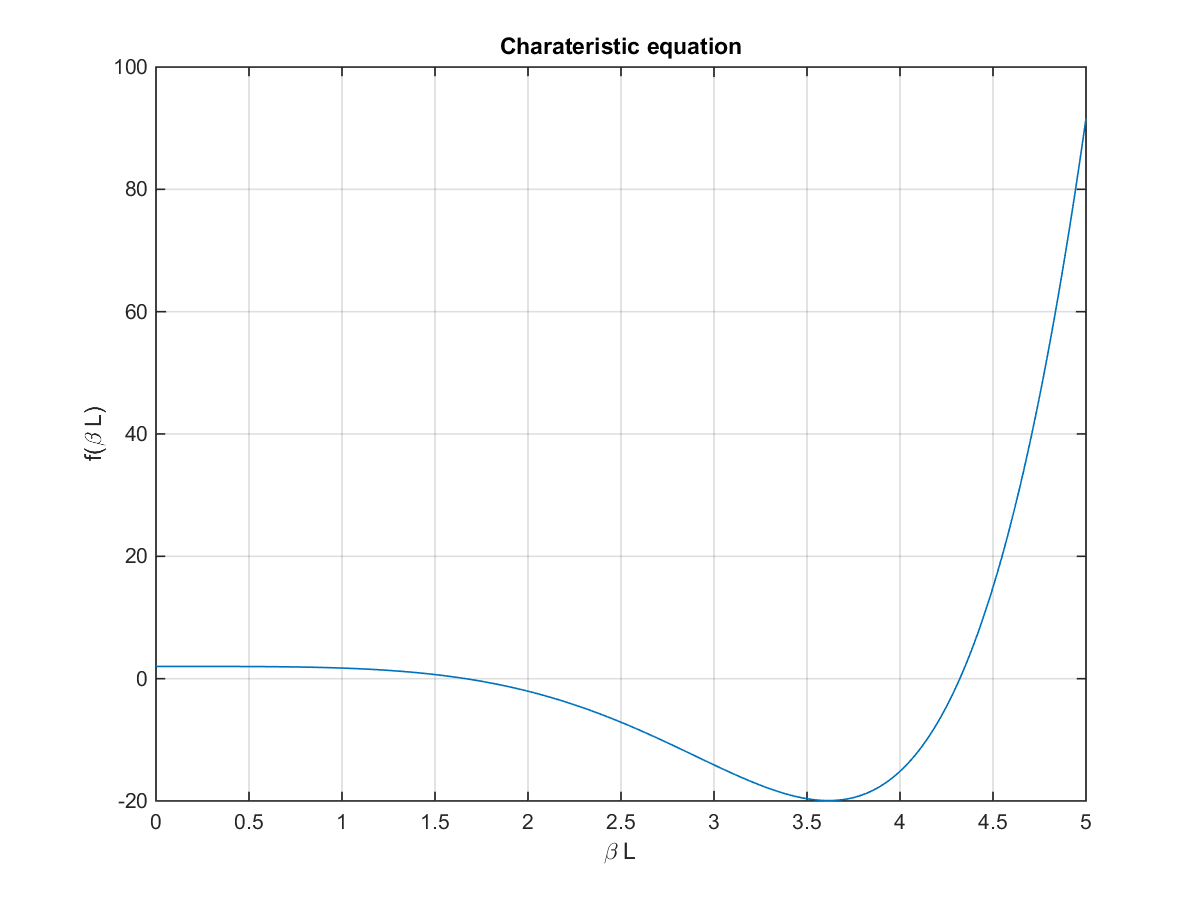
\includegraphics[scale=0.4]{fn1_VB1_1.png}
		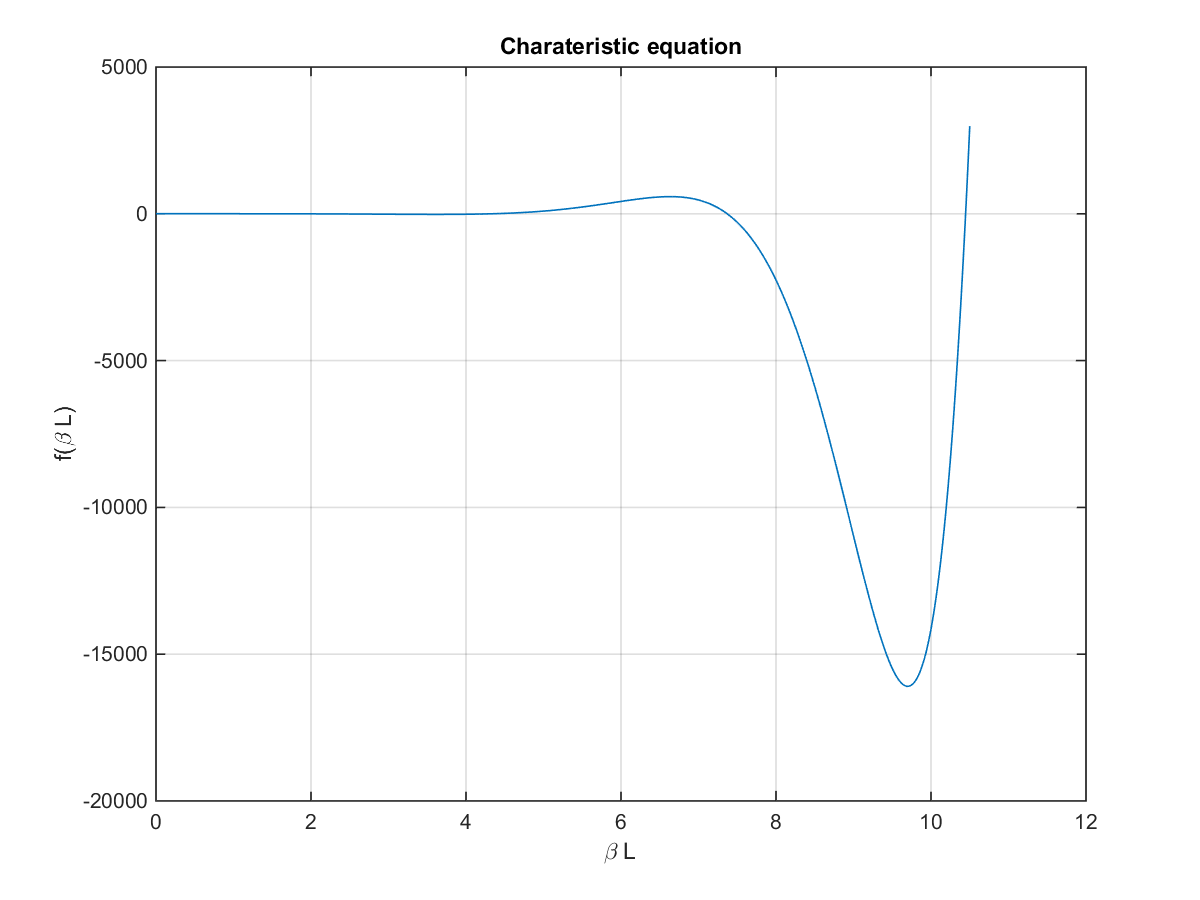
\includegraphics[scale=0.4]{fn1_VB1_2.png}
		\caption{Characteristic equation 1}
	\end{figure}\\
	The first four nonzero roots of characteristic equation are: $\beta_1L = 1.665, \beta_2L = 4.322, \beta_3L = 7.37 $ and $\beta_4L = 10.45$\\
	Natural frequencies is defined from computed values of $\beta$, we have:\\
	since: $ \beta^4 = \dfrac{\rho A\omega^2}{EI} \Rightarrow \omega = \beta^2\sqrt{\dfrac{EI}{\rho A}} = (\beta L)^2\sqrt{\dfrac{EI}{\rho AL^4}}$\\
	we first have: $\sqrt{\dfrac{EI}{\rho AL^4}} = \sqrt{\dfrac{68.9\bullet 10^9 \times 6.69\bullet 10^{-11}}{2.7\bullet10^6 \times 78.4\bullet10^{-6}\times 0.46^4}} \approx 0.7$\\
	\hspace*{1cm} $\beta_1L = 1.665 \Rightarrow \omega_1 = (\beta_1L)^2\bullet 0.7 = 1.665^2\bullet 0.7 = 1.94$ rad/s\\
	\hspace*{1cm} $\beta_2L = 4.322 \Rightarrow \omega_1 = (\beta_2L)^2\bullet 0.7 = 4.322^2\bullet 0.7 = 13.07$ rad/s\\
	\hspace*{1cm} $\beta_3L = 7.37 \Rightarrow \omega_1 = (\beta_3L)^2\bullet 0.7 = 7.37^2\bullet 0.7 = 38.02$ rad/s\\
	\hspace*{1cm} $\beta_4L = 10.45 \Rightarrow \omega_1 = (\beta_4L)^2\bullet 0.7 = 10.45^2\bullet 0.7 = 76.4$ rad/s\\
	The mode shape can be written as:\\
	$\bar{Y}_i(X) = \left(\dfrac{A}{B}\right)_i\left(\cosh(\beta_iL\dfrac{X}{L}) - \cos(\beta_iL\dfrac{X}L)\right) + \sinh(\beta_iL\dfrac{X}{L}) - \sin(\beta_iL\dfrac{X}{L})$\\
	with: 	$\left(\dfrac{A}{B}\right)_i =  -\dfrac{ \sinh\beta_iL + \sin \beta_iL}{\cosh \beta_iL + \cos \beta_iL} $\\
	we have the table result:
	\begin{tabular} {c c c c c}
		$\beta L$ & 1.575 & 4.226 & 7.282 & 10.371 \\
		$a/b$ & -1.341 & -0.985 & -1.0005 & 1
	\end{tabular}\\
	$\bar{Y}_1(X) = -1.341\left(\cosh(1.665\dfrac{X}{0.46}) - \cos(1.665\dfrac{X}{0.46})\right) + \sinh(1.665\dfrac{X}{0.46}) - \sin(1.6655\dfrac{X}{0.46})$\\	
	\hspace*{0.9cm} $= -1.341\left(\cosh(3.62X) - \cos(3.62X)\right) + \sinh(3.62X) - \sin(3.62X)$\\	
	$\bar{Y}_2(X) = -0.985\left(\cosh(4.322\dfrac{X}{0.46}) - \cos(4.322\dfrac{X}{0.46})\right) + \sinh(4.322\dfrac{X}{0.46}) - \sin(4.322\dfrac{X}{0.46})$\\	
	\hspace*{0.9cm} $= -0.985\left(\cosh(9.4X) - \cos(9.4X)\right) + \sinh(9.4X) - \sin(9.4X)$\\
	$\bar{Y}_3(X) = -1.0005\left(\cosh(7.37\dfrac{X}{0.46}) - \cos(7.37\dfrac{X}{0.46})\right) + \sinh(7.37\dfrac{X}{0.46}) - \sin(7.37\dfrac{X}{0.46})$\\	
	\hspace*{0.9cm} $= -1.0005\left(\cosh(16.02X) - \cos(16.02X)\right) + \sinh(16.02X) - \sin(16.02X)$\\
	$\bar{Y}_4(X) = -1\left(\cosh(10.45\dfrac{X}{0.46}) - \cos(10.45\dfrac{X}{0.46})\right) + \sinh(10.45\dfrac{X}{0.46}) - \sin(10.45\dfrac{X}{0.46})$\\	
	\hspace*{0.9cm} $= -\cosh(22.72X) + \cos(22.71X) + \sinh(22.72X) - \sin(22.72X)$\\
	\pagebreak
	
	Mode shape for the point mass:
	\begin{figure}[htp]
		\centering
		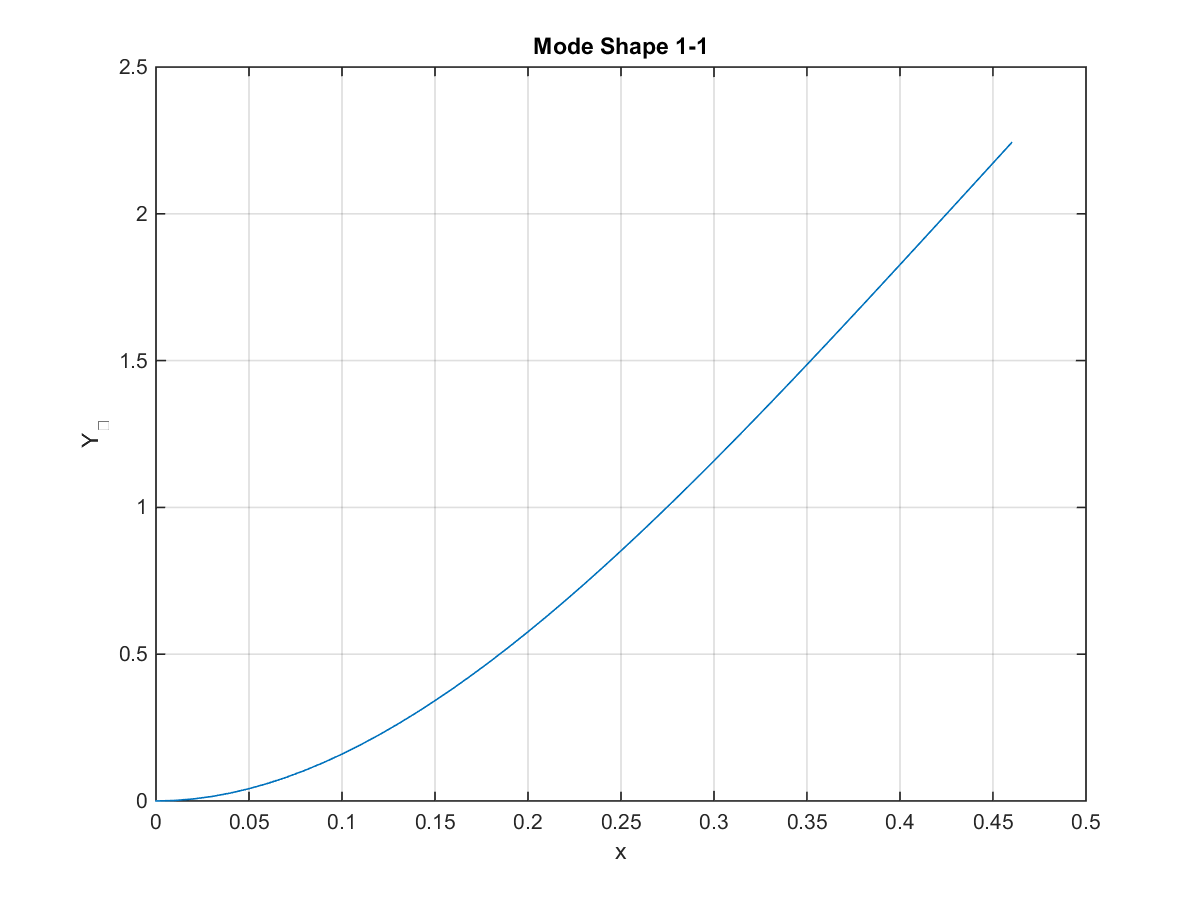
\includegraphics[scale=0.4]{fn1_VB1_mode1.png}
		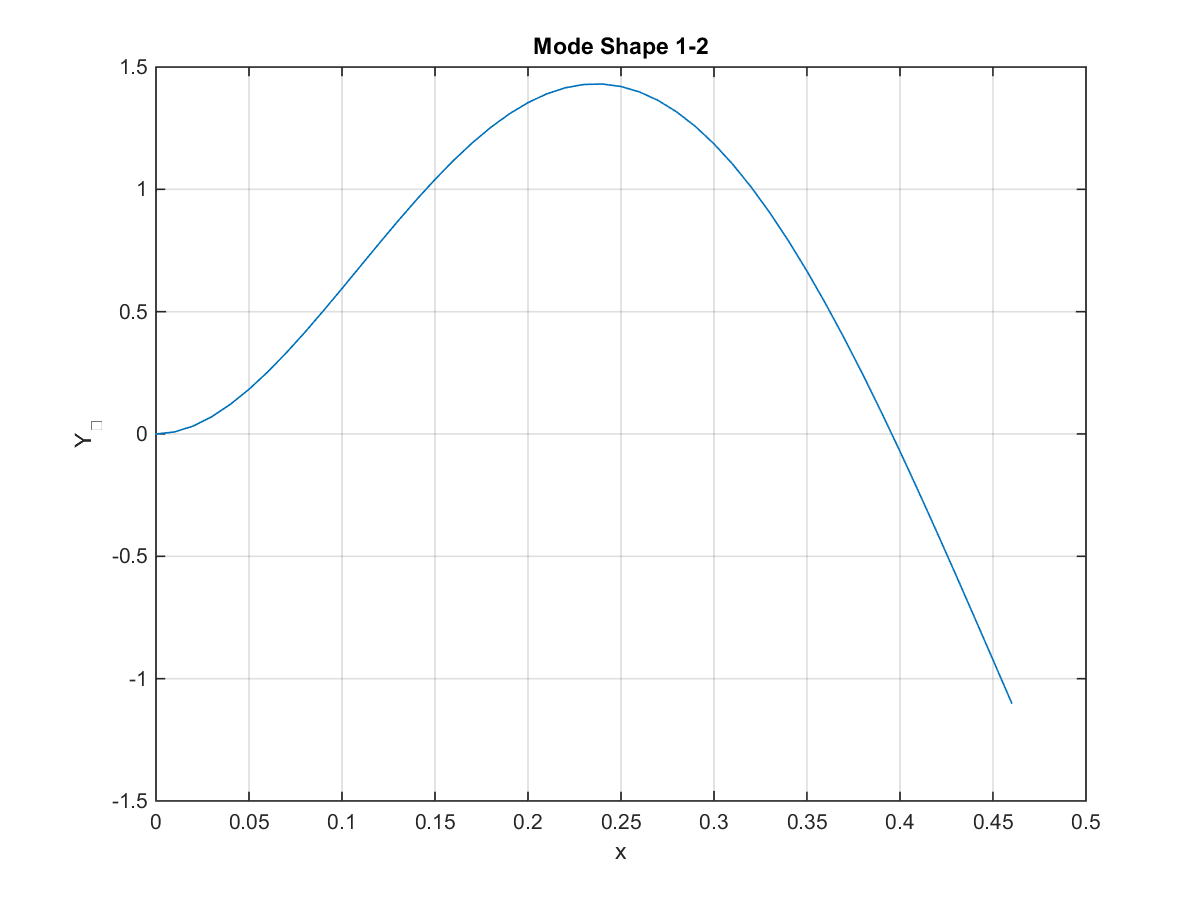
\includegraphics[scale=0.4]{fn1_VB1_mode2.png}
		\caption{Mode Shape 1 and 2}
	\end{figure}
	\begin{figure}[htp]
		\centering
		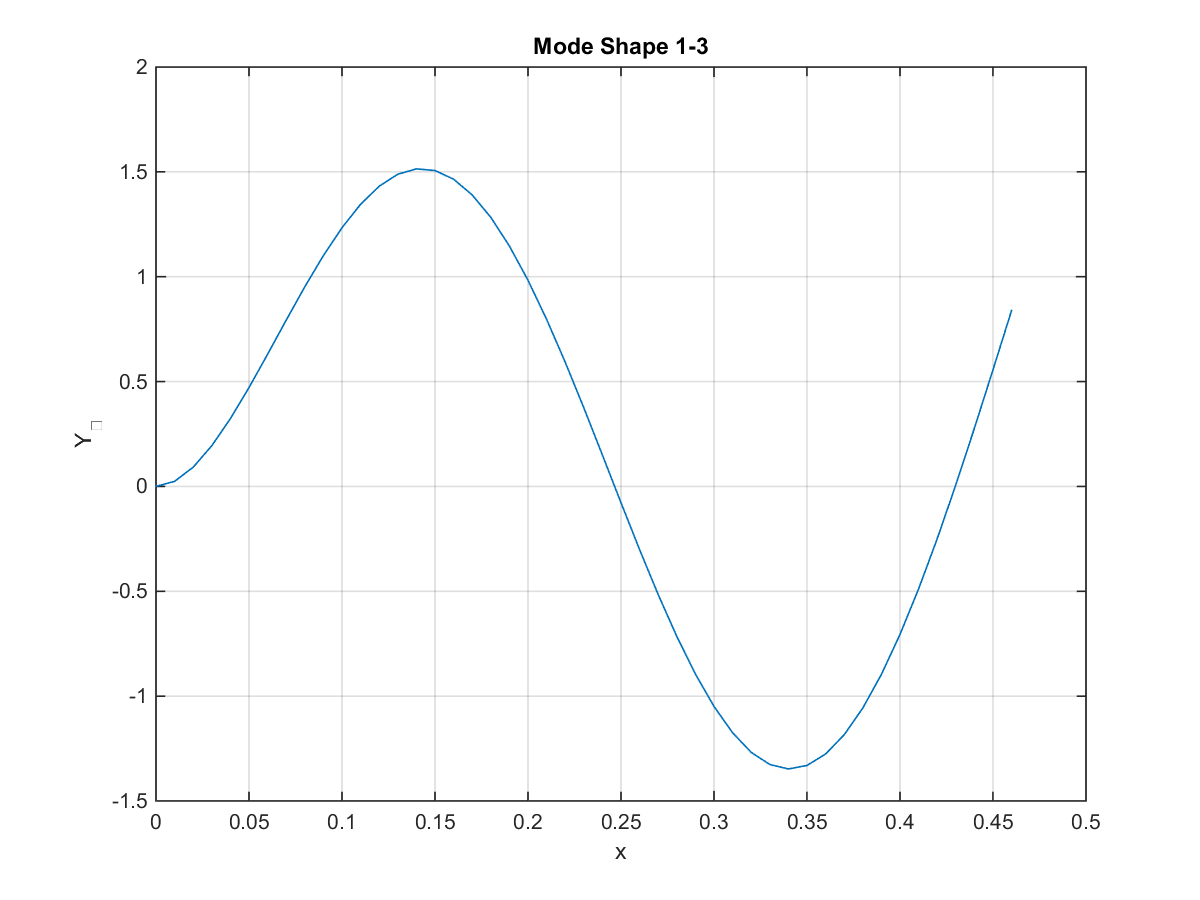
\includegraphics[scale=0.4]{fn1_VB1_mode3.png}
		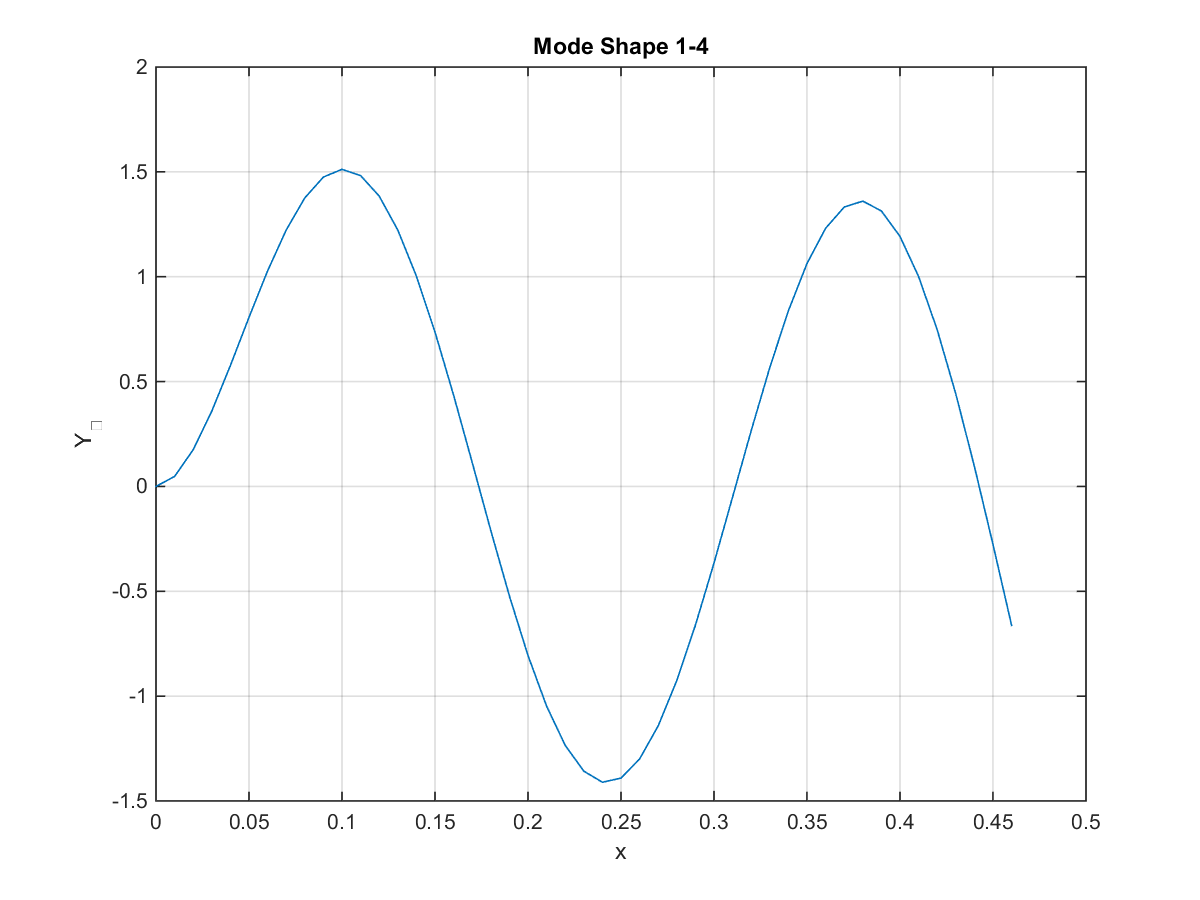
\includegraphics[scale=0.4]{fn1_VB1_mode4.png}
		\caption{Mode Shape 3 and 4}
	\end{figure}
		
	\item Modeled the tip mass as a solid having mass and inertia:\\
	- The first two bound conditions are same with above: we have equation (3) and (4)\\
	- From the rotational inertial we form the third and forth condition:\\
	\hspace*{2cm} $\dfrac{a}{b} = -\dfrac{k_1(\sinh\beta L - \sin\beta L) + (\cosh\beta L + \cos\beta L)}{k_1(\cosh\beta L + \cos\beta L) + (\sinh\beta L - \sin\beta L)}$	\hspace{2cm} (7)\\	
	\hspace*{2cm} $\dfrac{a}{b} = -\dfrac{k_2(\cosh\beta L - \cos\beta L) - (\sinh\beta L + \sin\beta L)}{k_2(\sinh\beta L + \sin\beta L) - (\cosh\beta L + \cos\beta L)}$ \hspace{2cm} (8)\\
	with $k_1 = \dfrac{\bar{M}}{m}\beta L = 0.1508\beta L$\\
	The rotary inertia is: $I_0 = \dfrac{1}{4}M_1r_1^2 + \dfrac{1}{3}M_1h_1^2 + M_2h_2^2$\\
	\hspace*{3.8cm} $ = \pi*1.15^2\times10^{-4}*1.13\times10^{-2}*2.7\times10^6\left( \dfrac{1}{4}1.15^2\times10^{-4} + \dfrac{1}{3}1.13^2\times10^{-4}\right) \\ \hspace*{4.4cm} + \pi*0.45^2\times10^{-4}*1.17\times10^{-2}*2.7\times10^6*1.17^2\times10^{-4}$\\
	\hspace*{3.8cm} $ = 1.234\times 10^{-3}$ \\
	So the rotary term for $k_2$ is: $k_2 = \dfrac{I_0}{mL^2}(\beta L)^3 = \dfrac{1.234\times10^{-3}}{97.4\times10^{-3}*0.46^2}(\beta L)^3 = 0.06(\beta L)^3 $\\
	Characteristic equation:\\
	$(k_1k_2-1)(\cosh\beta L\cos\beta L) - (k_1k_2 +1) + (k_1 + k_2)(\cosh\beta L\sin\beta L) -(k_1-k_2)(\sinh\beta L\cos\beta L) = 0 \\
	\Leftrightarrow (9.048\times10^{-3}(\beta )^4-1)(\cosh\beta L\cos\beta L) - (9.048\times10^{-3}(\beta )^4+1) + (0.1508\beta L + 0.06(\beta L)^3)(\cosh\beta L\sin\beta L) - (0.1508\beta L - 0.06(\beta L)^3)(\sinh\beta L\cos\beta L) = 0$ 
	\begin{figure}[htp]
		\centering
		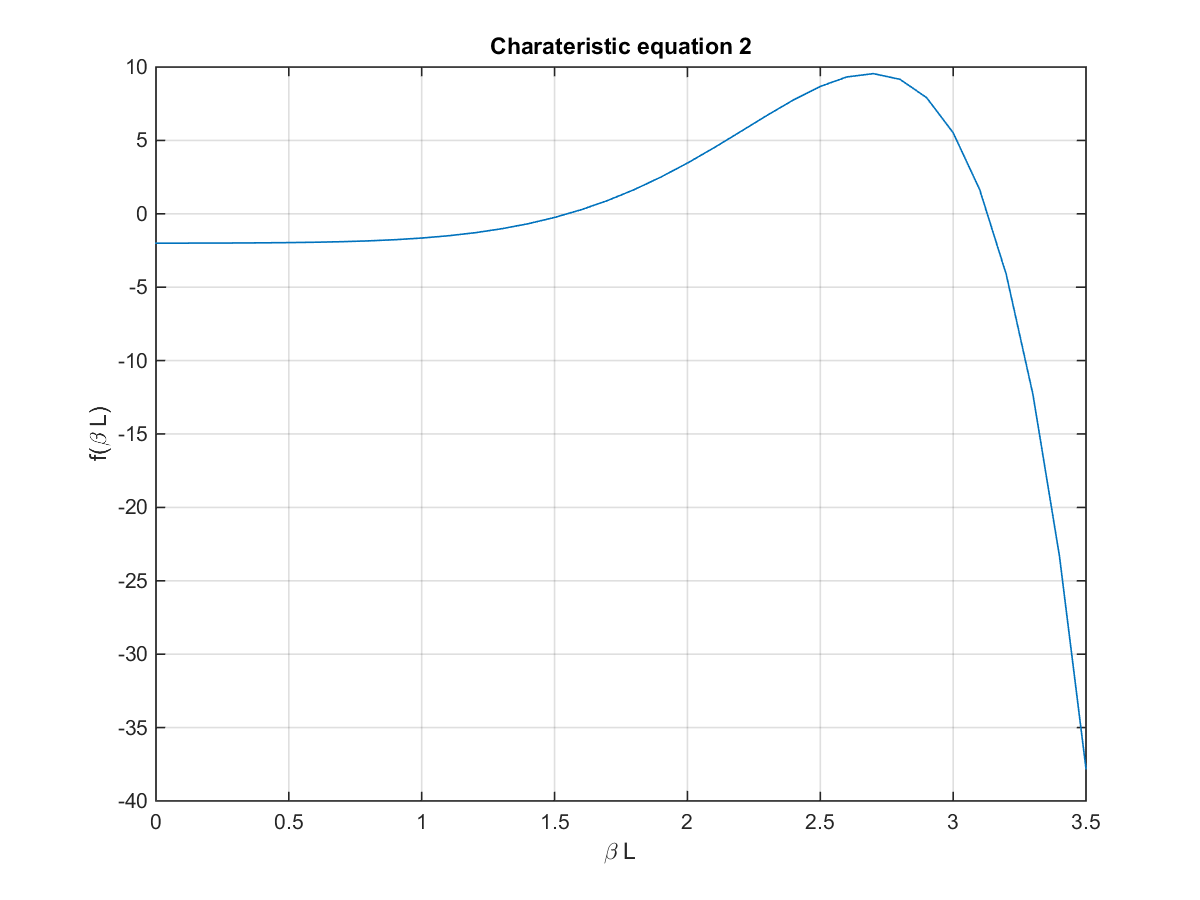
\includegraphics[scale=0.4]{fn1_VB2_1.png}
		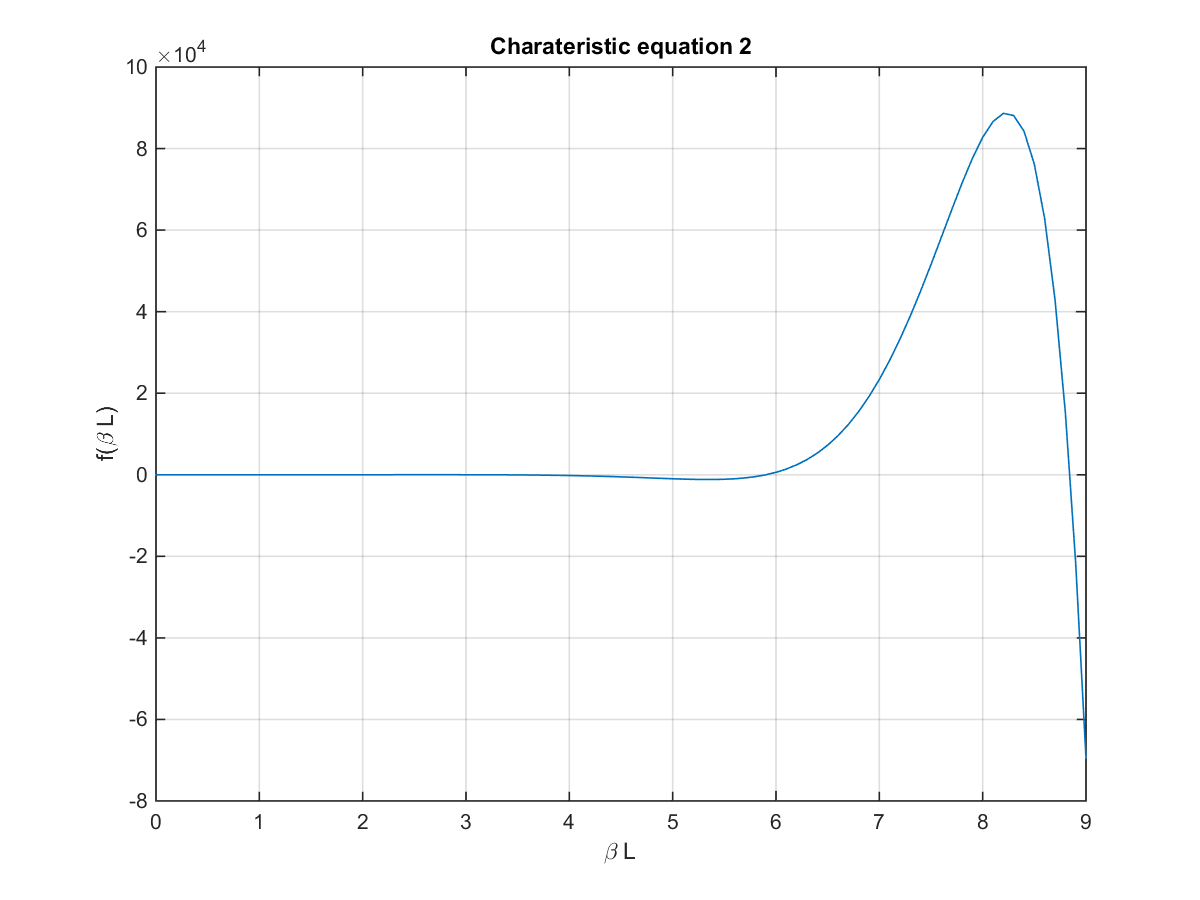
\includegraphics[scale=0.4]{fn1_VB2_2.png}
		\caption{Characteristic equation 2}
	\end{figure}\\
	The first four nonzero roots of characteristic equation are: $\beta_{21}L = 1.55, \beta_{22}L = 3.13, \beta_{23}L = 5.9 $ and $\beta_{24}L = 8.84$\\
	Natural frequencies is defined from computed values of $\beta$, we have: \\
	\hspace*{3cm} $\omega_n^2 = \beta^4\dfrac{EIL}{m} \Leftrightarrow \omega_n = (\beta L)^2\sqrt{\dfrac{EI}{mL^3}}$\\
	with: \hspace{1cm} 	$\sqrt{\dfrac{EI}{mL^3}} = \sqrt{\dfrac{68.9\bullet 10^9 \times 6.69\bullet 10^{-11}}{97.4\bullet10^{-3}\times 0.46^3}} \approx 22.05$\\
	The first four natural frequencies of vibration are defined:
	\begin{center}
		\begin{tabular} {c c c c c}
			$\beta L$ & 1.55 & 3.13 & 5.9 & 8.84 \\
			$\omega_n$ & 53 & 216.3 & 767.9 & 1725
		\end{tabular}
	\end{center}
	The mode shape can be written as:\\
	$\bar{Y}_i(X) = \left(\dfrac{A}{B}\right)_i\left(\cosh(\beta_iL\dfrac{X}{L}) - \cos(\beta_iL\dfrac{X}L)\right) + \sinh(\beta_iL\dfrac{X}{L}) - \sin(\beta_iL\dfrac{X}{L})$\\
	with: 	$\left(\dfrac{a}{b}\right)_i = -\dfrac{k_{1i}(\sinh\beta_iL - \sin\beta_iL) + (\cosh\beta_iL + \cos\beta_iL)}{k_{1i}(\cosh\beta_iL + \cos\beta_iL) + (\sinh\beta_iL - \sin\beta_iL)}$\\
	we have the table result:
	\begin{tabular} {c c c c c}
		$\beta L$ & 1.55 & 3.13 & 5.9 & 8.84 \\
		$a/b$ & -1.52 & -0.97 & -1.0002 & 1
	\end{tabular}\\
	$\bar{Y}_1(X) = -1.52\left(\cosh(1.55\dfrac{X}{0.46}) - \cos(1.55\dfrac{X}{0.46})\right) + \sinh(1.55\dfrac{X}{0.46}) - \sin(1.55\dfrac{X}{0.46})$\\	
	\hspace*{0.9cm} $= -1.52\left(\cosh(3.37X) - \cos(3.37X)\right) + \sinh(3.37X) - \sin(3.37X)$\\	
	$\bar{Y}_2(X) = -0.97\left(\cosh(3.13\dfrac{X}{0.46}) - \cos(3.13\dfrac{X}{0.46})\right) + \sinh(3.13\dfrac{X}{0.46}) - \sin(3.13\dfrac{X}{0.46})$\\	
	\hspace*{0.9cm} $= -0.97\left(\cosh(6.8X) - \cos(6.8X)\right) + \sinh(6.8X) - \sin(6.8X)$\\
	$\bar{Y}_3(X) = -1.0002\left(\cosh(5.9\dfrac{X}{0.46}) - \cos(5.9\dfrac{X}{0.46})\right) + \sinh(5.9\dfrac{X}{0.46}) - \sin(5.9\dfrac{X}{0.46})$\\	
	\hspace*{0.9cm} $= -1.0002\left(\cosh(12.83X) - \cos(12.83X)\right) + \sinh(12.83X) - \sin(12.83X)$\\
	$\bar{Y}_4(X) = -1\left(\cosh(8.84\dfrac{X}{0.46}) - \cos(8.84\dfrac{X}{0.46})\right) + \sinh(8.84\dfrac{X}{0.46}) - \sin(8.84\dfrac{X}{0.46})$\\	
	\hspace*{0.9cm} $= -\cosh(19.22X) + \cos(19.22X) + \sinh(19.22X) - \sin(19.22X)$
	\pagebreak
	
	Mode shape for the mass with int...:
	\begin{figure}[htp]
		\centering
		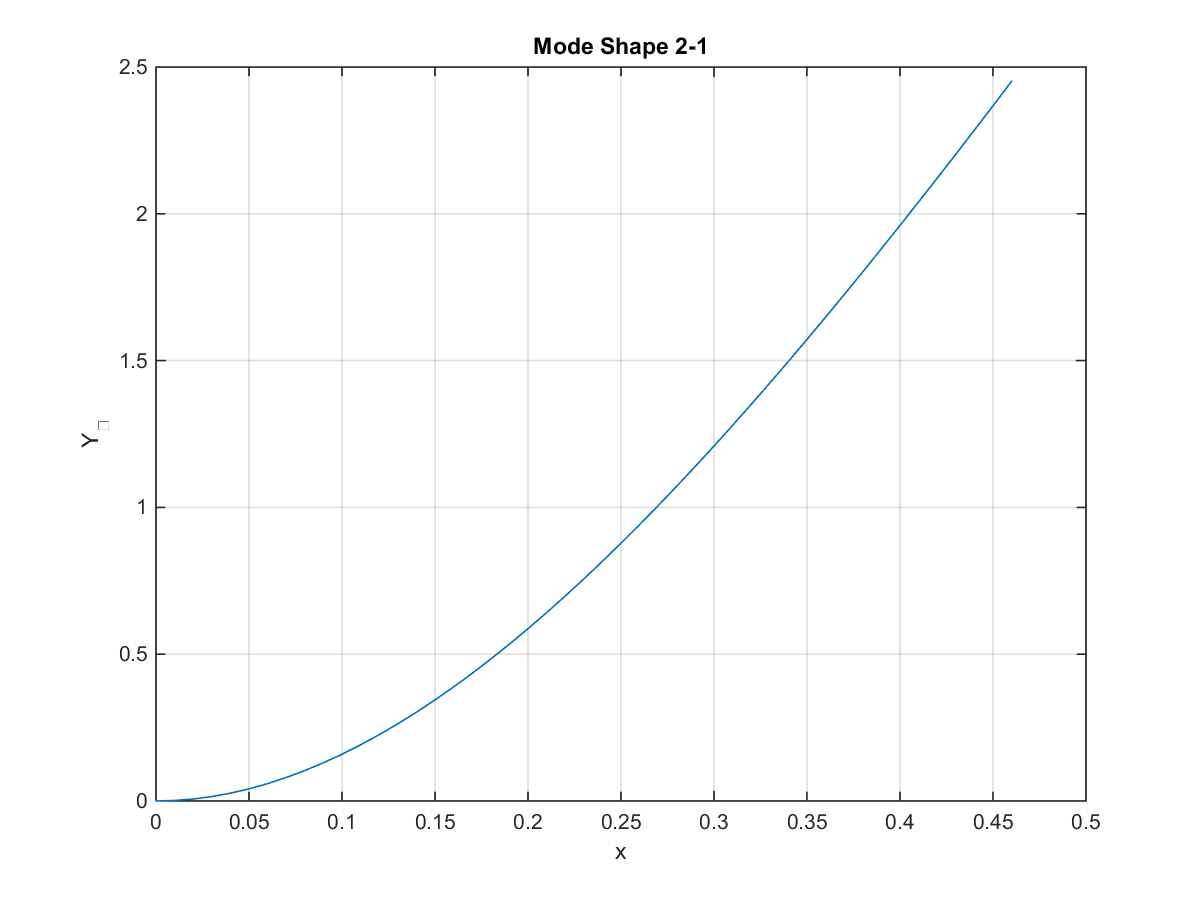
\includegraphics[scale=0.4]{fn1_VB2_mode1.png}
		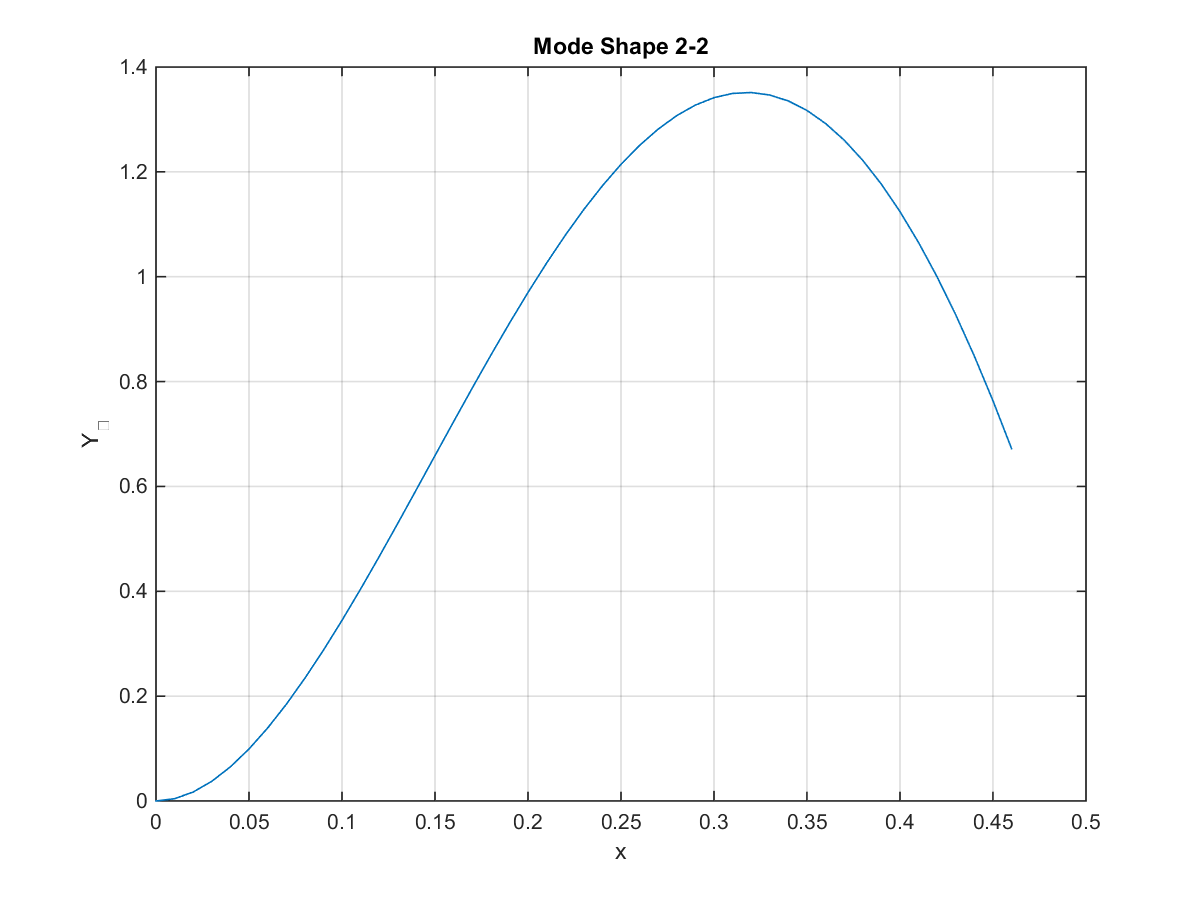
\includegraphics[scale=0.4]{fn1_VB2_mode2.png}
		\caption{Mode Shape 1 and 2}
	\end{figure}
	\begin{figure}[htp]
		\centering
		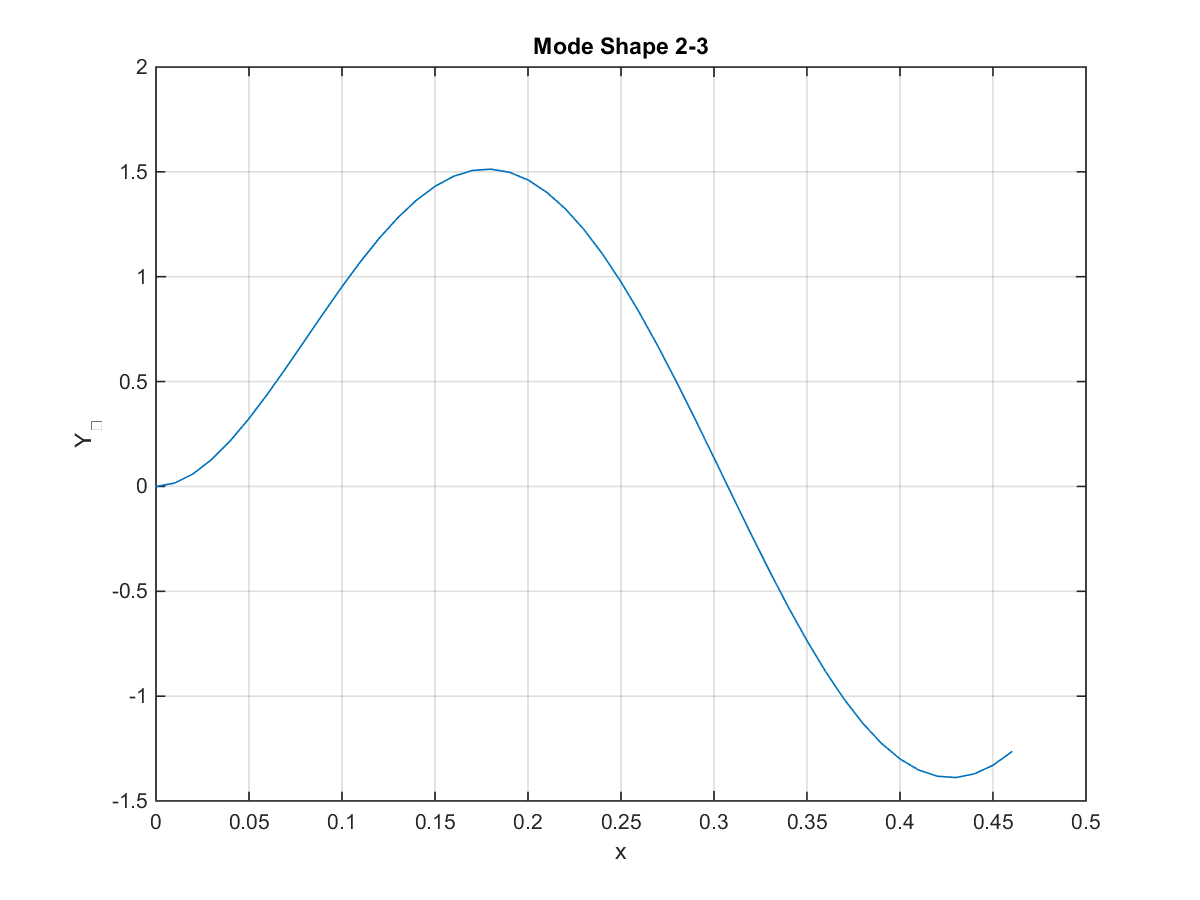
\includegraphics[scale=0.4]{fn1_VB2_mode3.png}
		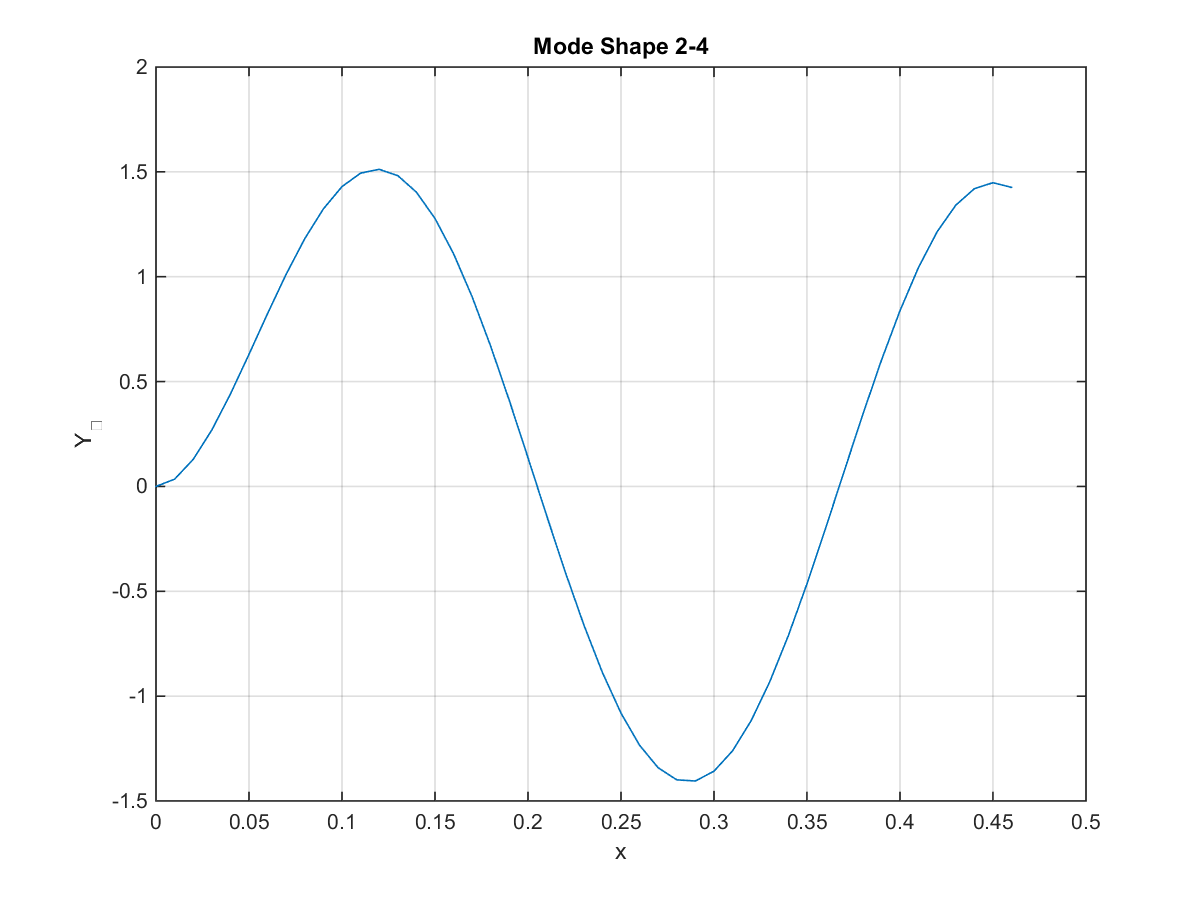
\includegraphics[scale=0.4]{fn1_VB2_mode4.png}
		\caption{Mode Shape 3 and 4}
	\end{figure}	
\end{enumerate}

\textbf{Problem 2.} Consider the given cantilever beam:
\begin{enumerate}
	\item Determine the first and second mode shapes and natural frequencies using the closed form solution:\\
	Applied result from \textbf{Problem 1} we have the general solution is equation (2):\\
	\hspace*{3cm}  $\bar{Y}(X) = a\cosh \beta X + b\sinh \beta X + c\cos \beta X + d\sin \beta X $ \hspace{2cm} (2)\\
	The boundary conditions are defined as:\\
	- End displacement (on left): $Y(0,t) = 0 \Rightarrow \bar{Y}(0) = 0 \Leftrightarrow \bar{Y}(0) = a + c = 0$ \hspace{2cm} (9)\\
	- End slope (on left): $Y'(0,t) = 0 \Rightarrow \bar{Y}'(0) = 0$\\
	\hspace*{1.6cm} with $ \bar{Y}'(X,t) = \beta a \sinh \beta X + \beta b \cosh \beta X - \beta c \sin \beta X + \beta d \cos \beta X $\\
	\hspace*{1.6cm} $\Rightarrow \bar{Y}'(0,t) = \beta b + \beta d = 0 \Leftrightarrow b + d = 0$ \hspace{5.8cm} (10) \\
	- End moment (on right): $ M(L,t) = EI\dfrac{\partial^2Y}{\partial X^2} (L,t) = 0 \Leftrightarrow \bar{Y}''(L,t) = 0$\\
	\hspace*{1.6cm} with $ \bar{Y}''(X,t) = \beta^2 a \cosh \beta X + \beta^2 b \sinh \beta X - \beta^2 c \cos \beta X - \beta^2 d \sin \beta X $\\
	\hspace*{1cm} $\Rightarrow \bar{Y}''(L,t) = \beta^2 \left(a \cosh \beta L + b \sinh \beta L - c \cos \beta L - d \sin \beta L \right) = 0 $\\
	\hspace*{2.7cm} $\Leftrightarrow a \cosh \beta L + b \sinh \beta L - c \cos \beta L - d \sin \beta L = 0 $ \hspace{1cm} (because $\beta \neq 0$) \\
	\hspace*{2.7cm} $ \Leftrightarrow \dfrac{a}{b} = -\dfrac{ \sinh\beta L + \sin \beta L}{\cosh \beta L + \cos \beta L} $ \hspace{6.5cm} (11)\\ 
	- Shear force $V$ at right end: $V(L,t) = \bar{M}Y''(L,t) \Leftrightarrow \bar{Y}'''(L,t) = 0$\\
	\hspace*{1.6cm} with: $ \bar{Y}'''(X,t) = \beta^3 a \sinh \beta X + \beta^3 b \cosh \beta X + \beta^3 c \sin \beta X - \beta^3 d \cos \beta X $\\
	\hspace*{1cm} $\Rightarrow \bar{Y}'''(L,t) = \beta^3 \left(a \sinh \beta L + b \cosh \beta L + c \sin \beta L - d \cos \beta L\right) = 0$ \\ 
	\hspace*{2.8cm} $\Leftrightarrow a(\sinh\beta L - \sin\beta L) = -b(\cosh\beta L + \cos\beta L)$\\
	\hspace*{2.8cm} $\Leftrightarrow \dfrac{a}{b} = -\dfrac{(\cosh\beta L + \cos\beta L)}{(\sinh\beta L - \sin\beta L)} $ \hspace{6.1cm} (12) \\
	From (11) and (12) we have characteristic equation:\\
	\hspace*{1cm} $ \dfrac{ \sinh\beta L + \sin \beta L}{\cosh \beta L + \cos \beta L} = \dfrac{(\cosh\beta L + \cos\beta L)}{(\sinh\beta L - \sin\beta L)} \Leftrightarrow \cosh\beta L \sin\beta L + 1 = 0 $\\
	\begin{figure}[htp]
		\centering
		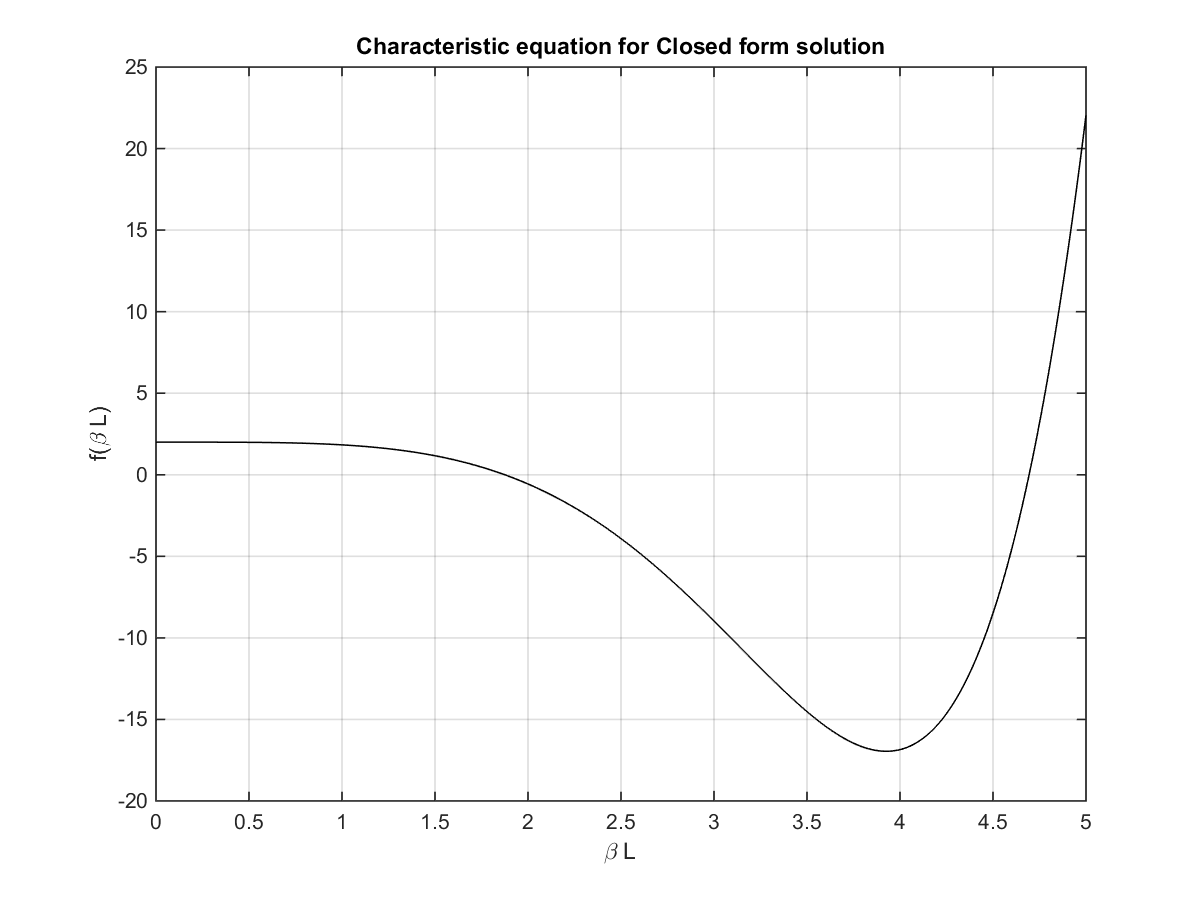
\includegraphics[scale=0.5]{fn2_VB1_1.png}
		\caption{Characteristic equation}
	\end{figure}\\
	The first 2 nonzero roots of characteristic equation are: $\beta_1L = 1.8751, \beta_2L = 4.4941$\\
	Natural frequencies is defined from computed values of $\beta$, we have:\\
	since: $ \beta^4 = \dfrac{\rho A\omega^2}{EI} \Rightarrow \omega = \beta^2\sqrt{\dfrac{EI}{\rho A}} = (\beta L)^2\sqrt{\dfrac{EI}{\rho AL^4}}$\\
	we first have: $\sqrt{\dfrac{EI}{\rho AL^4}} = \sqrt{\dfrac{68.9\bullet 10^9 \times 6.69\bullet 10^{-11}}{2.7\bullet10^6 \times 78.4\bullet10^{-6}\times 0.46^4}} \approx 22.0499$\\
	\hspace*{1cm} $\beta_1L = 1.665 \Rightarrow \omega_1 = (\beta_1L)^2\bullet 22.0499 = 1.8751^2\bullet 22.0499 = 77.53$ rad/s\\
	\hspace*{1cm} $\beta_2L = 4.322 \Rightarrow \omega_1 = (\beta_2L)^2\bullet 22.0499 = 4.6941^2\bullet 22.0499 = 485.86$ rad/s
	
	The mode shape can be written as:\\
	$\bar{Y}_i(X) = \left(\dfrac{A}{B}\right)_i\left(\cosh(\beta_iL\dfrac{X}{L}) - \cos(\beta_iL\dfrac{X}L)\right) + \sinh(\beta_iL\dfrac{X}{L}) - \sin(\beta_iL\dfrac{X}{L})$\\
	with: 	$\left(\dfrac{A}{B}\right)_i =  -\dfrac{ \sinh\beta_iL + \sin \beta_iL}{\cosh \beta_iL + \cos \beta_iL} $\\
	we have the table result:
	\begin{tabular} {c c c}
		$\beta L$ & 1.8751 & 4.6941 \\
		$a/b$ & -1.3622 & -0.9819 
	\end{tabular}\\
	$\bar{Y}_1(X) = -1.3622\left(\cosh(1.8751\dfrac{X}{0.46}) - \cos(1.8751\dfrac{X}{0.46})\right) + \sinh(1.8751\dfrac{X}{0.46}) - \sin(1.8751\dfrac{X}{0.46})$\\	
	\hspace*{0.9cm} $= -1.3622\left(\cosh(4.0763X) - \cos(4.0763X)\right) + \sinh(4.0763X) - \sin(4.0763X)$\\	
	$\bar{Y}_2(X) = -0.9819\left(\cosh(4.6941\dfrac{X}{0.46}) - \cos(4.6941\dfrac{X}{0.46})\right) + \sinh(4.6941\dfrac{X}{0.46}) - \sin(4.6941\dfrac{X}{0.46})$\\	
	\hspace*{0.9cm} $= -0.985\left(\cosh(10.2046X) - \cos(10.2046X)\right) + \sinh(10.2046X) - \sin(10.2046X)$\\
	
	\begin{figure}[htp]
		\centering
		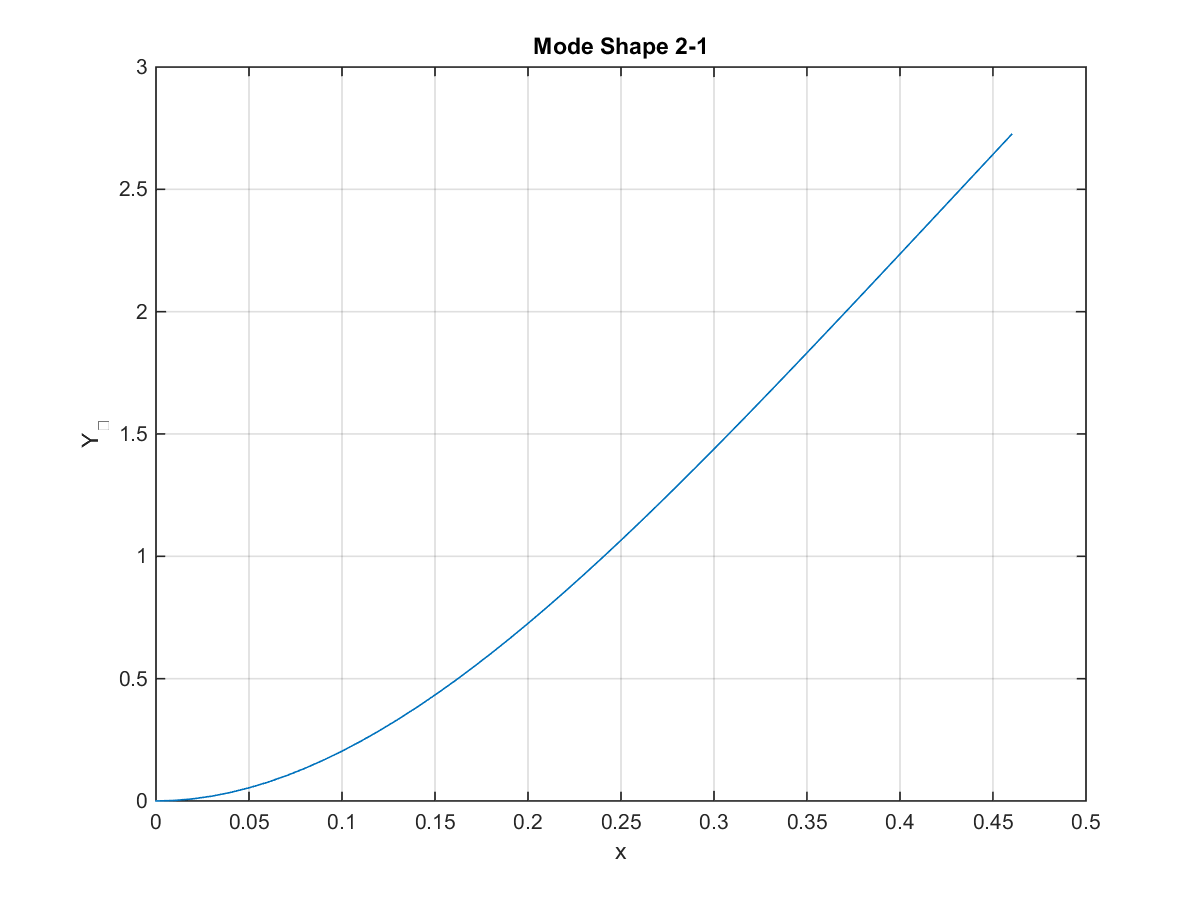
\includegraphics[scale=0.4]{fn2_VB1_mode1.png}
		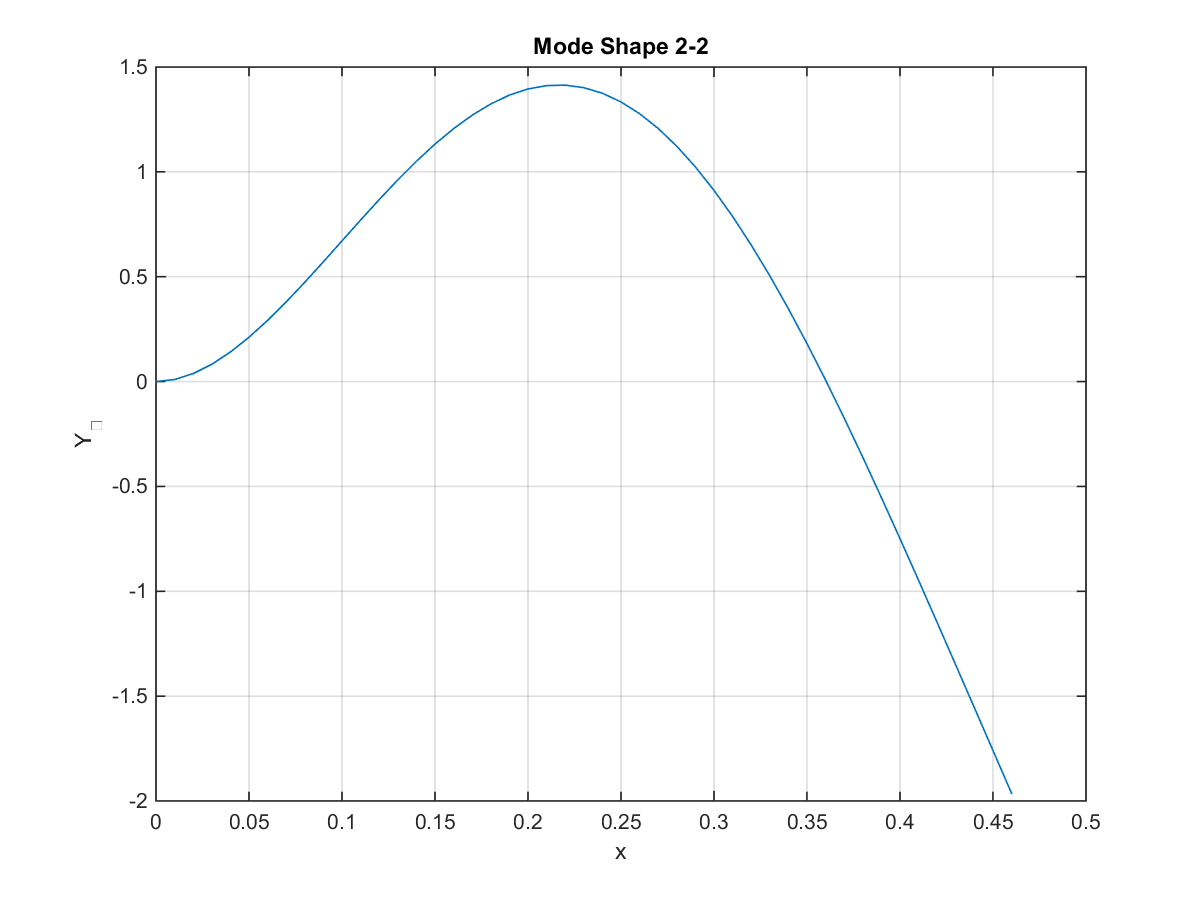
\includegraphics[scale=0.4]{fn2_VB1_mode2.png}
		\caption{Mode Shape 1 and 2 - no mass applied}
	\end{figure}
	
	\item Mode the beam with three finite elements:\\
	Beam is divided by three element and four-node mesh (length of each element is $l_e = 46/3$ cm). \\
	We will have 4 linear coordinates $u_1(t), u_3(t), u_5(t), u_7(t)$ and 4 rotational coordinates $u_2(t), u_4(t), u_6(t), u_8(t)$\\
	For each element, the transverse static displacement must satisfy: $\dfrac{\partial^2}{\partial x^2}\left[ EI\dfrac{\partial^2u(x,t)}{\partial x^2}\right] = 0$\\
	with: $u(x,t) = c_1(t)x^3 + c_2(t)x^2 + c_3(t)x + c_4(t)$\\
	\hspace{1cm} $c_i(t)$ are constants of integration with respect to spatial variable $x$\\
	The unknown nodal displacement $u_i(t)$ of each element must satisfy the boundary condition:\\
	$u(0,t) = u_1(t); u_x(0,t) = u_2(t); u(l_e,t) = u_3(t); u(l_e,t) = u_4(t)$\\
	\hspace*{2cm} $c_4(t) = u_1(t)$ \hspace{1cm} $c_3(t) = u_2(t)$\\
	\hspace*{2cm} $c_2(t) = \dfrac{1}{l_e^2}[3(u_3 -u_1) - l_e(2u_2 + u_4)]$\\
	\hspace*{2cm} $c_1(t) = \dfrac{1}{l_e^3}[2(u_1 -u_3) - l_e(u_2 + u_4)]$\\
	$\Rightarrow u(x,t) = \left[ 1 - 3\dfrac{x^2}{l_e^2} + 2\dfrac{x^3}{l_e^3} \right]u_1(t) + l_e\left[ \dfrac{x}{l_e} - 2\dfrac{x^2}{l_e^2} + \dfrac{x^3}{l_e^3}\right] u_2(t) + \left[ 3\dfrac{x^2}{l_e^2} -2\dfrac{x^3}{l_e^3}\right] u_3(t) + l_e\left[ -\dfrac{x^2}{l_e^2} + \dfrac{x^3}{l_e^3}\right] u_4(t)$\\
	
	For the first element:\\
	+ The kinetic energy of element: $T(t) = \dfrac{1}{2}\int_{0}^{l_e} \rho \textbf{A}[u_t(x,t)]^2\mathrm{d}x = \dfrac{1}{2}\dot{\textbf{u}}_1^TM\dot{\textbf{u}}_1$ \\
	with: $\textbf{u}_1(t) = \begin{bmatrix} u_1(t) \\ u_2(t) \\ u_3(t) \\ u_4(t) \end{bmatrix}$ \hspace{1cm} and \hspace{1cm} $ M = \dfrac{\rho \textbf{A}l_e}{420} \begin{bmatrix} 156 & 22l_e & 54 & -12l_e \\ 22l_e & 4l_e^2 & 13l_e & -3l_e^2 \\ 54 & 13l_e & 156 & -22l_e \\ -13l_e & -3l_e^2 & -22l_e & 4l_e^2 \end{bmatrix} $\\
	+ The strain energy is given by: $V(t) = \int_{0}^{l_e} EI[u_{xx}(x,t)]^2\mathrm{d}x = \dfrac{1}{2}\textbf{u}_1^TK\textbf{u}_1$\\
	when $\textbf{u}_1$ is defined above and $K = \dfrac{EI}{l_e^3} \begin{bmatrix} 12 & 6l_e & -12 & 6l_e \\ 6l_e & 4l_e^2 & -6l_e & 2l_e^2 \\ -12 & -6l_e & 12 & -6l_e \\ 6l_e & 2l_e^2 & -6l_e & 4l_e^2 \end{bmatrix} $
	The equation for the first element is:\\
	$M\ddot{\textbf{u}}_1 + K\textbf{u}_1 = \dfrac{\rho \textbf{A}l_e}{420} \begin{bmatrix} 156 & 22l_e & 54 & -12l_e \\ 22l_e & 4l_e^2 & 13l_e & -3l_e^2 \\ 54 & 13l_e & 156 & -22l_e \\ -13l_e & -3l_e^2 & -22l_e & 4l_e^2 \end{bmatrix} \begin{bmatrix} \ddot{u}_1(t) \\ \ddot{u}_2(t) \\ \ddot{u}_3(t) \\ \ddot{u}_4(t) \end{bmatrix} + \dfrac{EI}{l_e^3} \begin{bmatrix} 12 & 6l_e & -12 & 6l_e \\ 6l_e & 4l_e^2 & -6l_e & 2l_e^2 \\ -12 & -6l_e & 12 & -6l_e \\ 6l_e & 2l_e^2 & -6l_e & 4l_e^2 \end{bmatrix} \begin{bmatrix} u_1(t) \\ u_2(t) \\ u_3(t) \\ u_4(t) \end{bmatrix} =$\\
	Because the left end of rod is clamped so both the deflection and slope is 0, we have: $u_1 = u_2 =0$\\
	Equation (13) become:\\
	\hspace*{2cm} $\dfrac{\rho \textbf{A}l_e}{420} \begin{bmatrix} 156 & -22l_e \\ -22l_e & 4l_e^2 \end{bmatrix} \begin{bmatrix} \ddot{u}_3(t) \\ \ddot{u}_4(t) \end{bmatrix} + \dfrac{EI}{l_e^3} \begin{bmatrix} 12 & -6l_e \\ -6l_e & 4l_e^2 \end{bmatrix} \begin{bmatrix} u_3(t) \\ u_4(t) \end{bmatrix} = 0$ \hspace{2cm} (14) \\
	
	Similarity, we have for the second element:\\
	$M\ddot{\textbf{u}}_2 + K\textbf{u}_2 = \dfrac{\rho \textbf{A}l_e}{420} \begin{bmatrix} 156 & 22l_e & 54 & -12l_e \\ 22l_e & 4l_e^2 & 13l_e & -3l_e^2 \\ 54 & 13l_e & 156 & -22l_e \\ -13l_e & -3l_e^2 & -22l_e & 4l_e^2 \end{bmatrix} \begin{bmatrix} \ddot{u}_3(t) \\ \ddot{u}_4(t) \\ \ddot{u}_5(t) \\ \ddot{u}_6(t) \end{bmatrix} + \dfrac{EI}{l_e^3} \begin{bmatrix} 12 & 6l_e & -12 & 6l_e \\ 6l_e & 4l_e^2 & -6l_e & 2l_e^2 \\ -12 & -6l_e & 12 & -6l_e \\ 6l_e & 2l_e^2 & -6l_e & 4l_e^2 \end{bmatrix} \begin{bmatrix} u_3(t) \\ u_4(t) \\ u_5(t) \\ u_6(t) \end{bmatrix} =$\\
	
	For the third element:\\
	$M\ddot{\textbf{u}}_3 + K\textbf{u}_3 = \dfrac{\rho \textbf{A}l_e}{420} \begin{bmatrix} 156 & 22l_e & 54 & -12l_e \\ 22l_e & 4l_e^2 & 13l_e & -3l_e^2 \\ 54 & 13l_e & 156 & -22l_e \\ -13l_e & -3l_e^2 & -22l_e & 4l_e^2 \end{bmatrix} \begin{bmatrix} \ddot{u}_5(t) \\ \ddot{u}_6(t) \\ \ddot{u}_7(t) \\ \ddot{u}_8(t) \end{bmatrix} + \dfrac{EI}{l_e^3} \begin{bmatrix} 12 & 6l_e & -12 & 6l_e \\ 6l_e & 4l_e^2 & -6l_e & 2l_e^2 \\ -12 & -6l_e & 12 & -6l_e \\ 6l_e & 2l_e^2 & -6l_e & 4l_e^2 \end{bmatrix} \begin{bmatrix} u_5(t) \\ u_6(t) \\ u_7(t) \\ u_8(t) \end{bmatrix} =$\\
	
	From (14) (15) and (16) we have the global equation:\\
	$\dfrac{\rho \textbf{A}l_e}{420} \begin{bmatrix} 312 & 0 & 54 & -13                                                                    l_e & 0 & 0\\ 0 & 8l_e^2 & 13l_e & -3l_e^2&0&0 \\ 54 & 13l_e & 312 & 0 & 54 & -13l_e \\ -13l_e & -3l_e^2 & 0 & 8l_e^2 & 13l_e & -3l_e^2 \\ 0&0& 54 & 13l_e & 156 & -22l_e \\ 0&0& -13l_e & -3l_e^2 & -22l_e & 4l_e^2  \end{bmatrix} \begin{bmatrix} \ddot{u}_3(t) \\ \ddot{u}_4(t) \\ \ddot{u}_5(t) \\ \ddot{u}_6(t) \\ \ddot{u}_7(t) \\ \ddot{u}_8(t) \end{bmatrix} + \dfrac{EI}{l_e^3} \begin{bmatrix} 24 & 0 & -12 & 6l_e &0&0 \\ 0 & 8l_e^2 & -6l_e & 2l_e^2 &0&0 \\ -12 & -6l_e & 24 & 0 & -12 & 6l_e \\ 6l_e & 2l_e^2 & 0 & 8l_e^2 & -6l_e & 2l_e^2 \\ 0&0& -12 & -6l_e & 12 & -6l_e \\ 0&0& 6l_e & 2l_e^2 & -6l_e & 4l_e^2 \end{bmatrix} \begin{bmatrix} u_3(t) \\ u_4(t) \\ u_5(t) \\ u_6(t) \\ u_7(t) \\ u_8(t) \end{bmatrix}$\\
	Let $\textbf{u} = \textbf{x}e^{-\omega t}$, we have: $\ddot{\textbf{u}} = -\omega^2\textbf{x}e^{\omega t}$\\
	$\dfrac{\rho \textbf{A}l_e}{420} = \dfrac{2.7\bullet10^3 \times 3.2\bullet10^{-3} \times 2.45\bullet 10^{-2} \times 0.46}{3*420} = 0.00773$  \\
	and $\dfrac{EI}{l_e^3} = \dfrac{68.9\bullet 10^9 \times 6.69\bullet10^{-11} \times 3^3}{0.46^3} = 1278.6  $\\
	(17) will become: $\left(-\omega^2[\textbf{M}] + [\textbf{K}]\right)\textbf{x}e^{-\omega t} = 0$;\\
	Utilize \texttt{MATLAB} to solve this equation, we come up with two first natural frequency (value of $\omega$):\\
	$\omega_1 = 76.16$ and $\omega_2 = 478.81$\\
	\pagebreak
	
	Characteristic equation for matrix $\left[-\omega^2[\textbf{M}] + [\textbf{K}]\right]$
	\begin{figure}[htp]
		\centering
		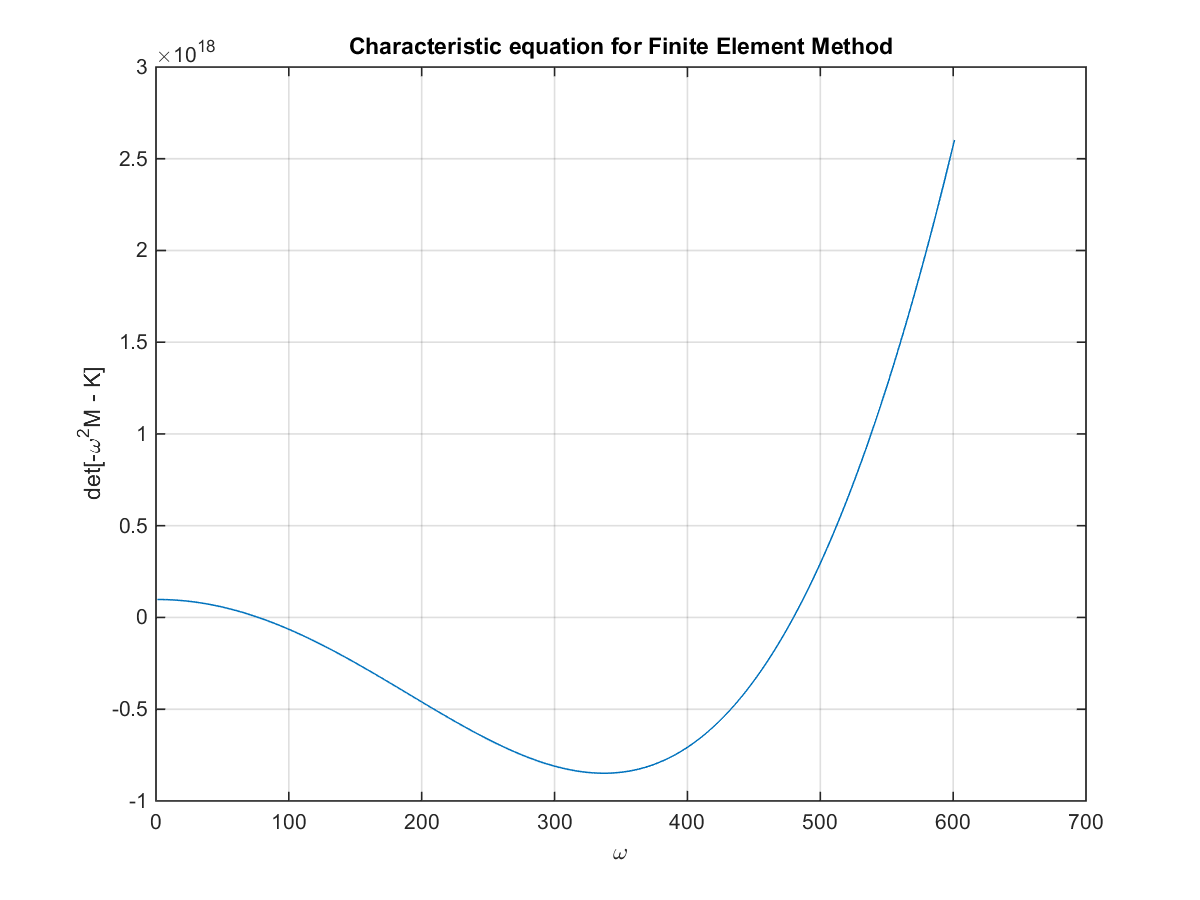
\includegraphics[scale=0.5]{fn2_VB2_1.png}
		\caption{Characteristic equation for finite element method}
	\end{figure}
	\begin{figure}[htp]
		\centering
		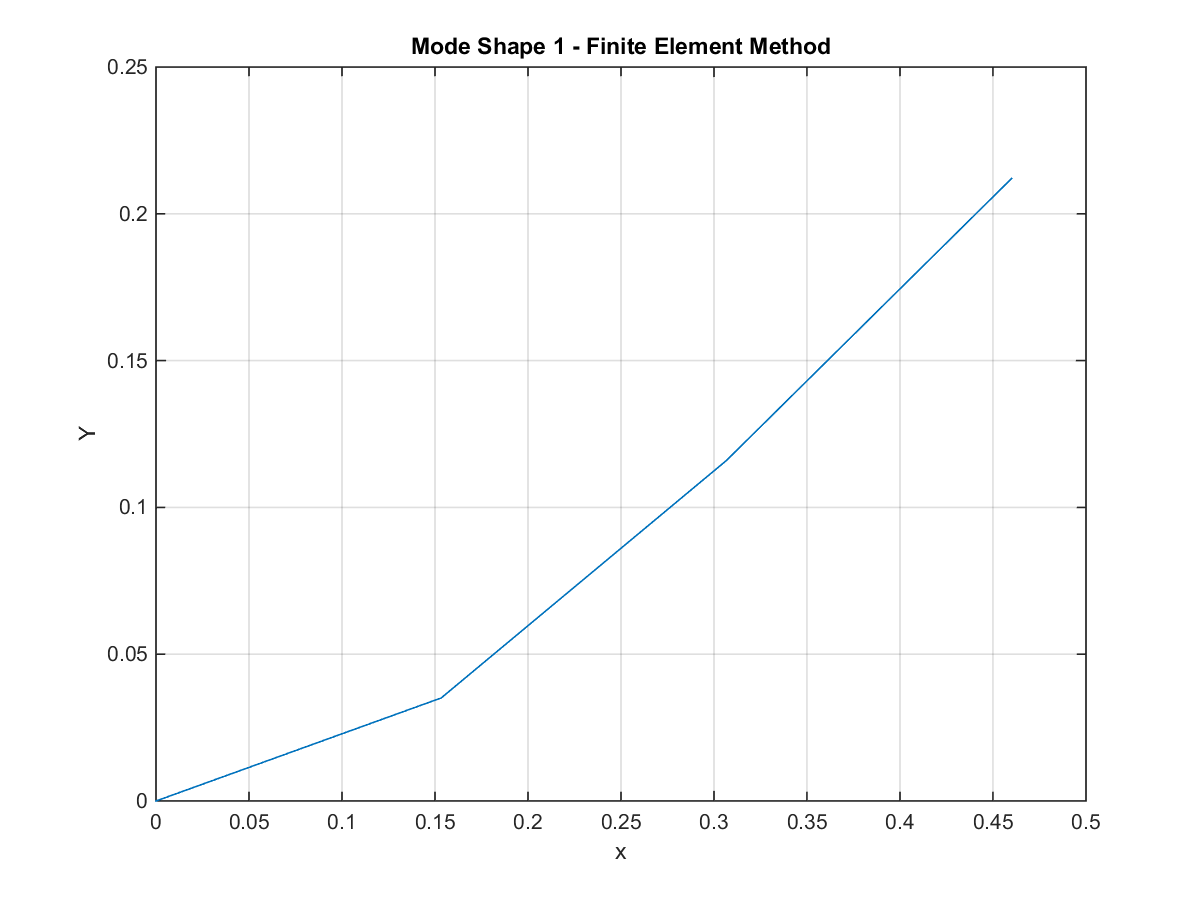
\includegraphics[scale=0.4]{fn2_VB2_3.png}
		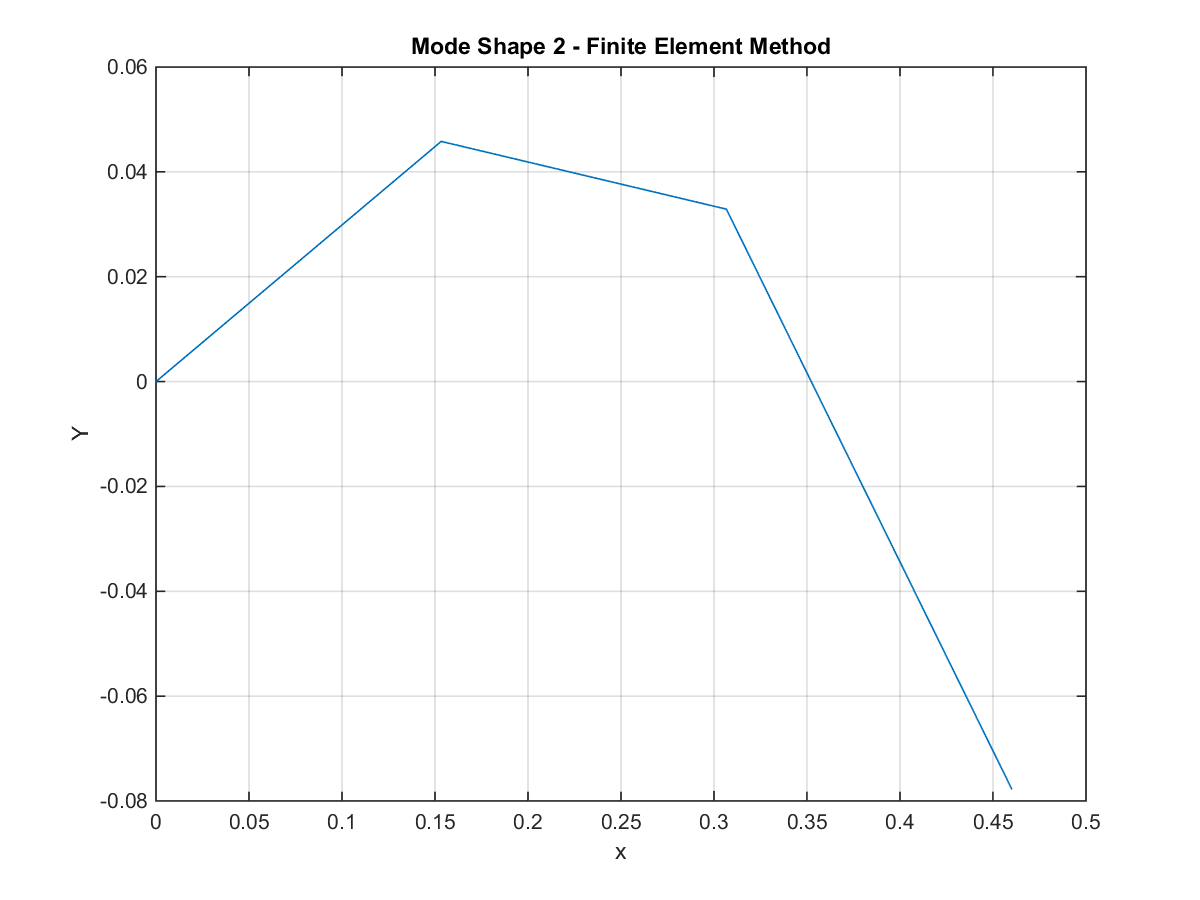
\includegraphics[scale=0.4]{fn2_VB2_4.png}
		\caption{Mode Shape 1 and 2 - no mass applied}
	\end{figure}
	\end{enumerate}
\pagebreak
\textbf{Problem 3.} Use Discrete Fourier Transform equation to transform the square wave data sample to the frequency domain:
\begin{enumerate}
	\item Use a sampling rate of 25 Hz ($\Delta t = 0.04$) over a 1-second sampling period and determine:\\
	The \textit{magnitude frequency} domain component up to the Nyquist frequency:
	\begin{figure}[htp]
		\centering
		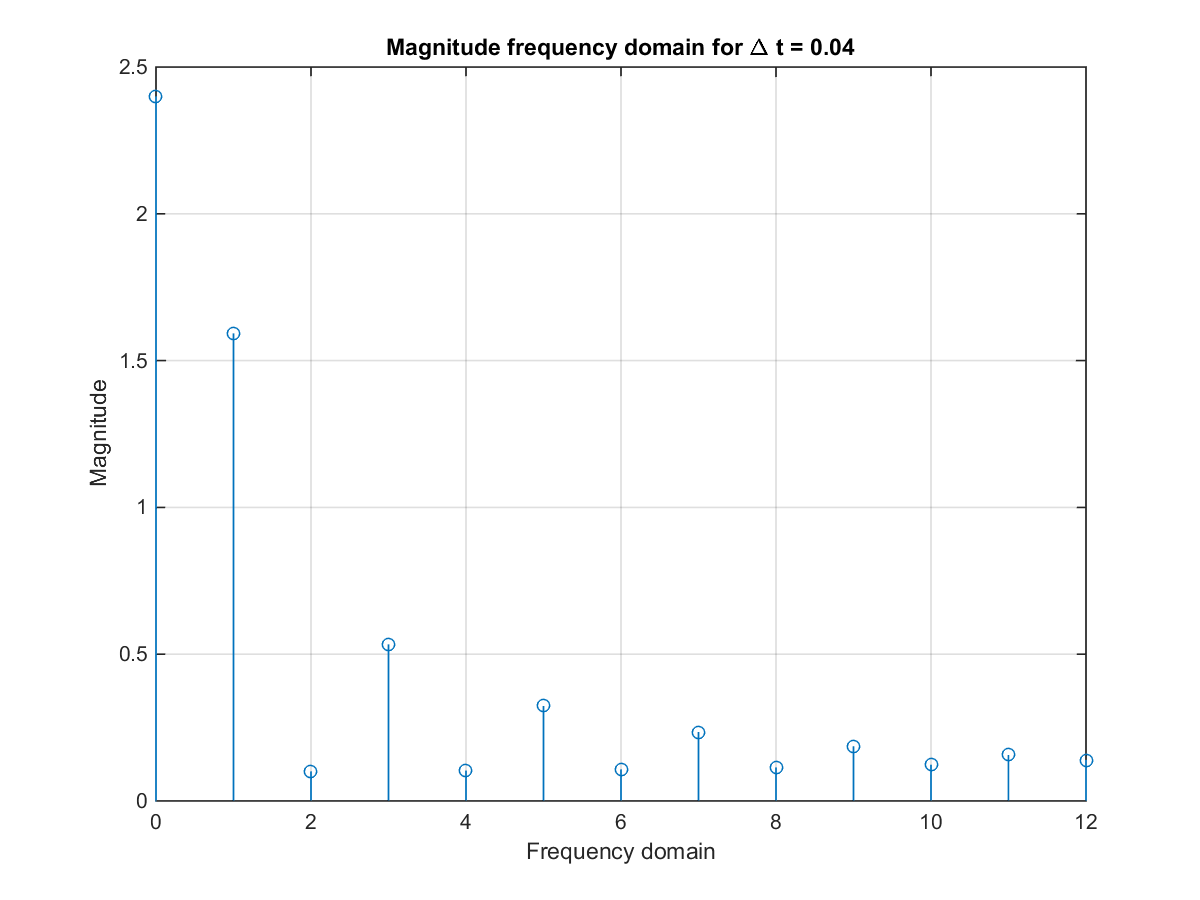
\includegraphics[scale=0.58]{fn3_VB1_1.png}
		\caption{The \textit{magnitude frequency} domain component  $\Delta t = 0.04$}
	\end{figure}
	The inverse discrete Fourier Transform (IDFT) using the harmonic component:
	\begin{figure}[htp]
		\centering
		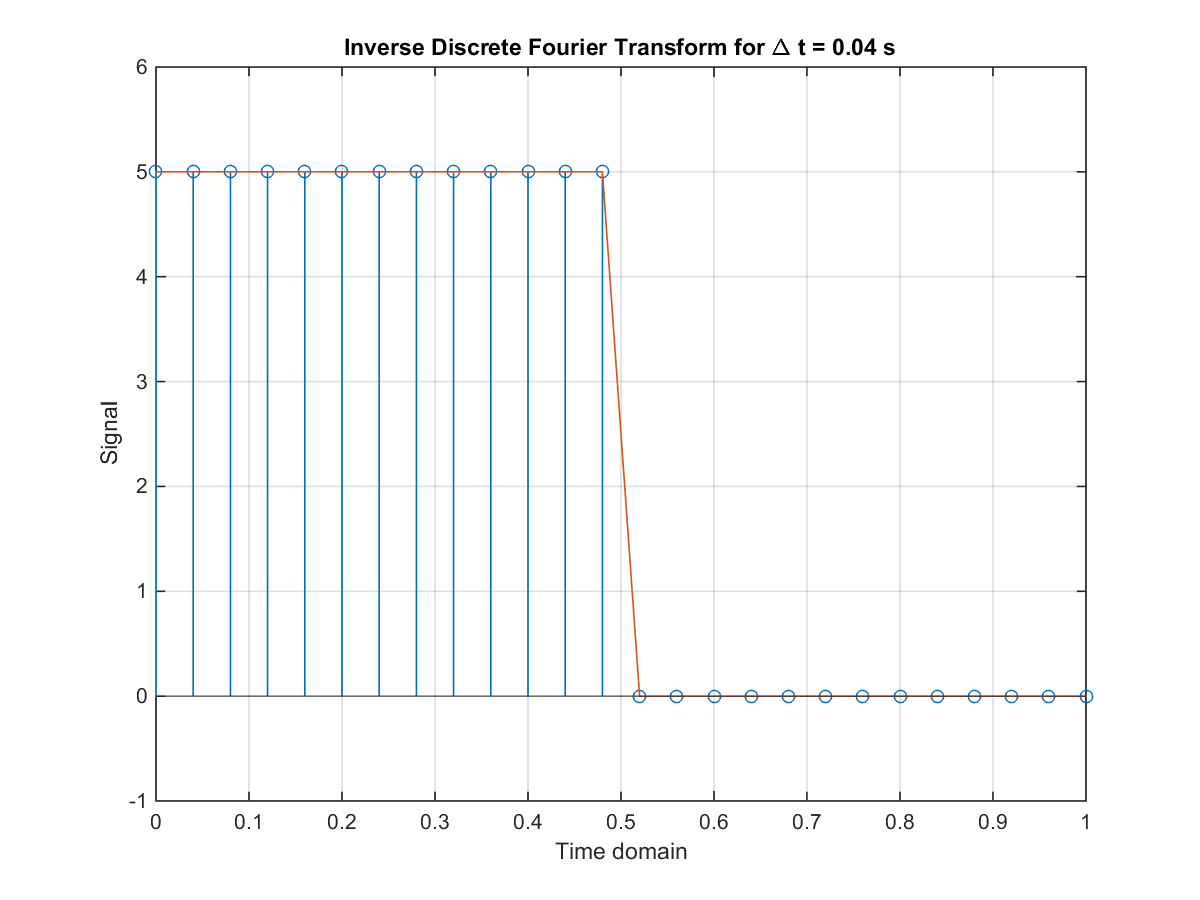
\includegraphics[scale=0.58]{fn3_VB1_2.png}
		\caption{The inverse discrete Fourier Transform for  $\Delta t = 0.04$}
	\end{figure}
	\pagebreak
	\item Change sampling rate to 16.67 Hz ($\Delta t = 0.06$):
	\begin{figure}[htp]
		\centering
		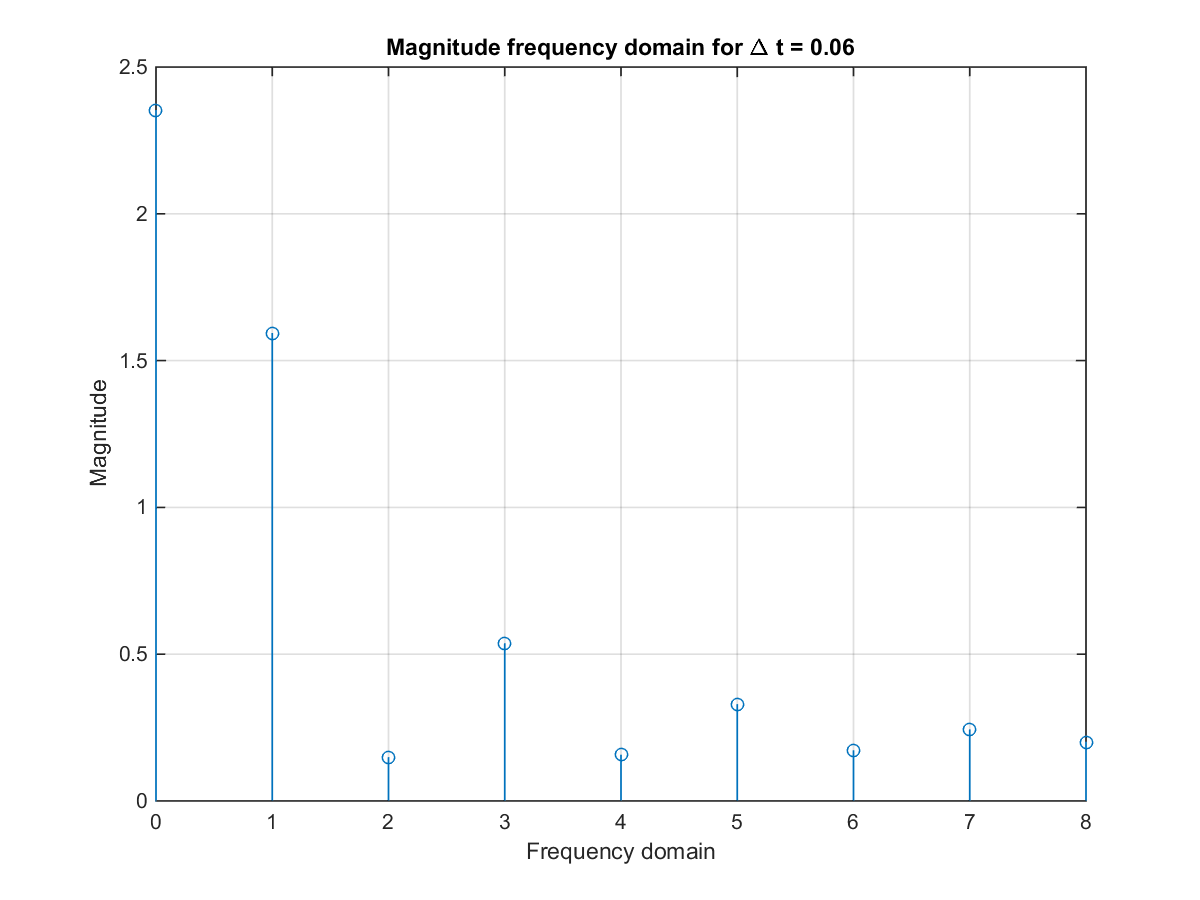
\includegraphics[scale=0.58]{fn3_VB2_1.png}
		\caption{The \textit{magnitude frequency} domain component  $\Delta t = 0.06$}
	\end{figure}\\
	The inverse discrete Fourier Transform (IDFT) using the harmonic component:
	\begin{figure}[htp]
		\centering
		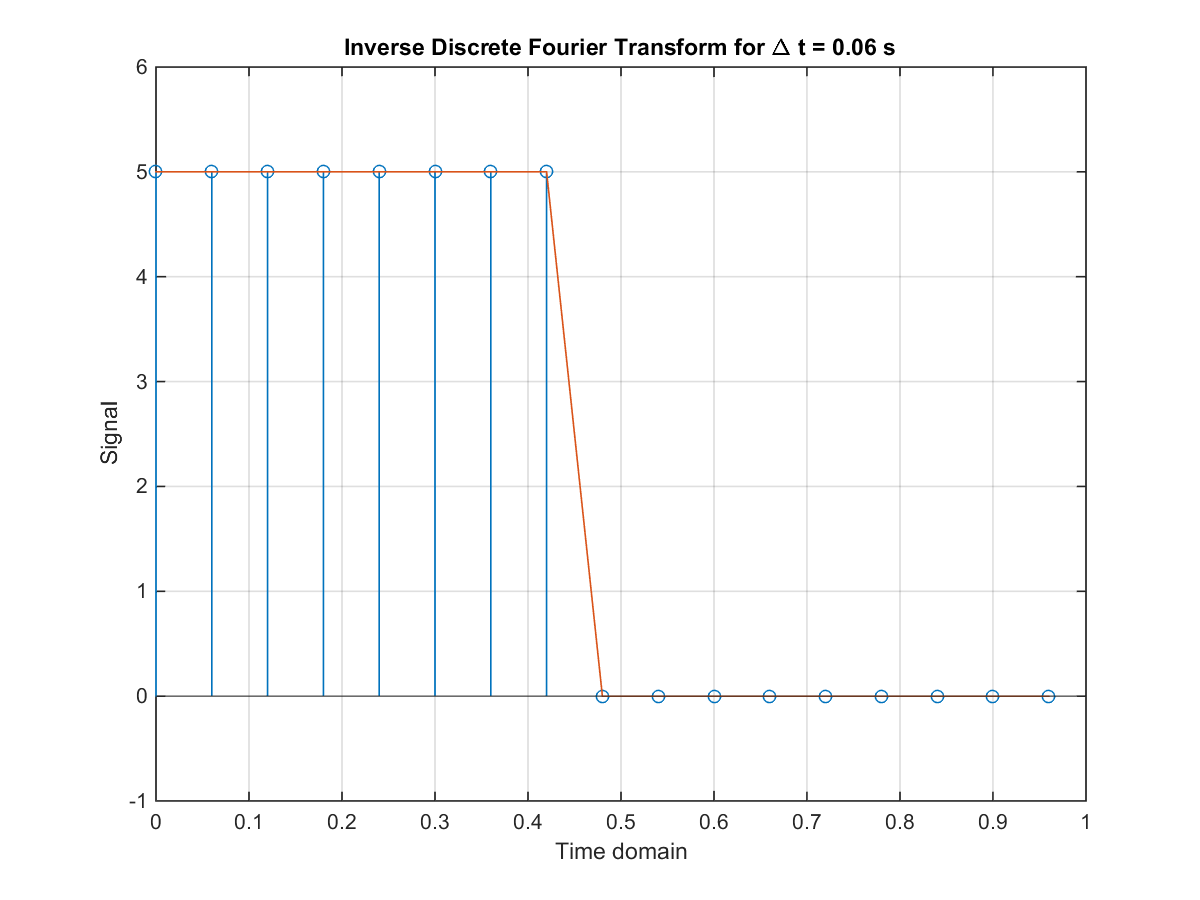
\includegraphics[scale=0.58]{fn3_VB2_2.png}
		\caption{The inverse discrete Fourier Transform for $\Delta t = 0.06$}
	\end{figure}\\
	\pagebreak
	
	When overlay frequency in both case:
	\begin{figure}[htp]
		\centering
		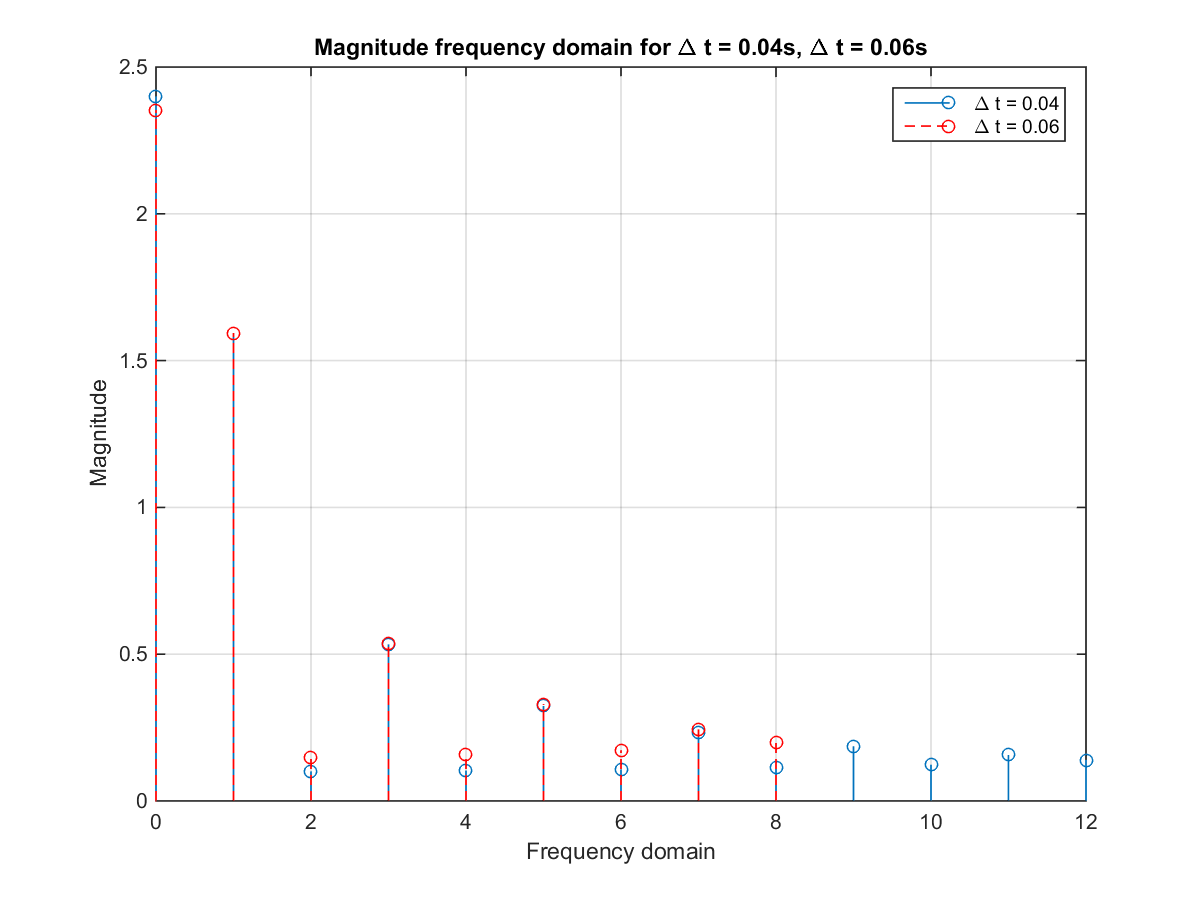
\includegraphics[scale=0.58]{fn3_VB2_3.png}
		\caption{The \textit{magnitude frequency} domain component: $\Delta t = 0.04$ and  $\Delta t = 0.06$}
	\end{figure}\\
	From above figure we see that with odd number (on frequency domain) we have no leakage, with even number (on frequency domain), we will have leakage (it seems increasing).\\
	The inverse discrete Fourier Transform (IDFT) using the harmonic component:
	\begin{figure}[htp]
		\centering
		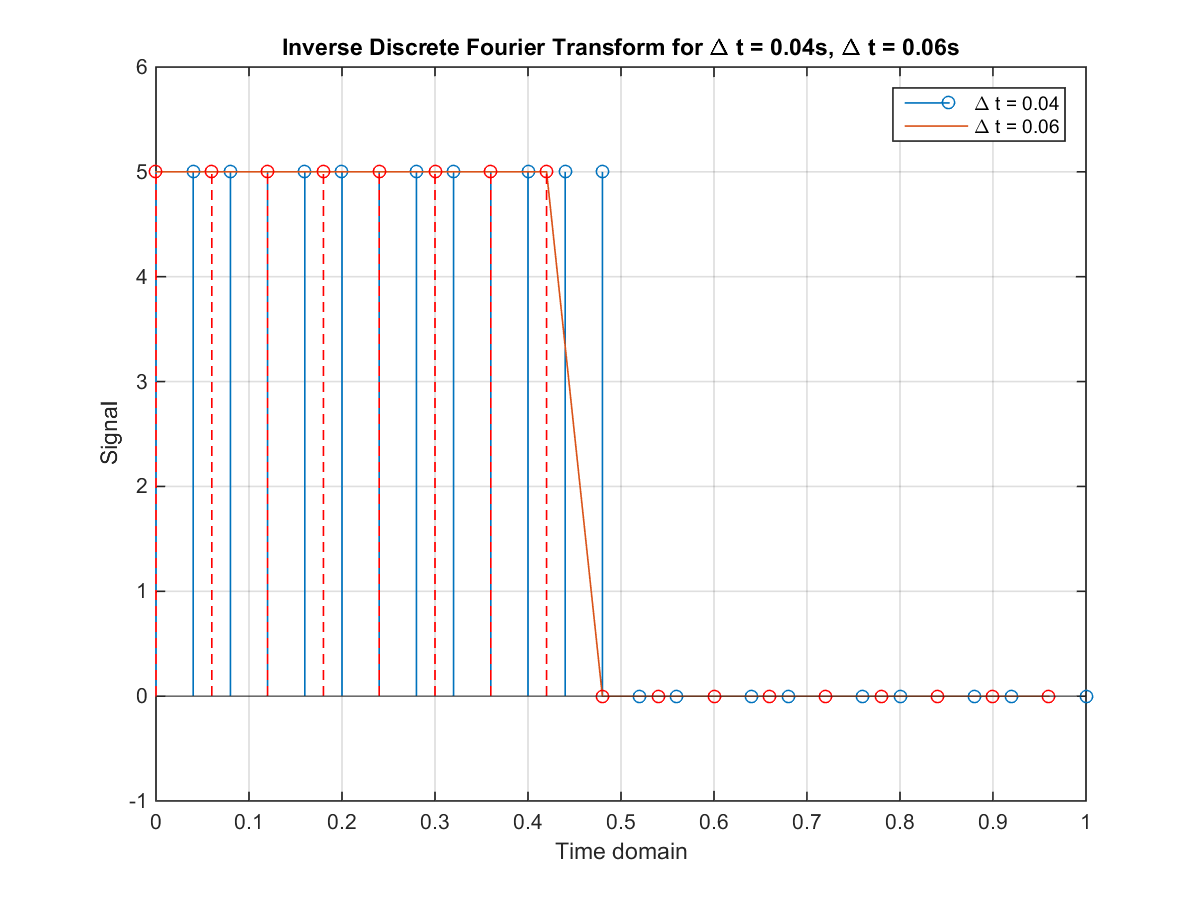
\includegraphics[scale=0.58]{fn3_VB2_4.png}
		\caption{The inverse discrete Fourier Transform for $\Delta t = 0.04$ and $\Delta t = 0.06$}
	\end{figure}\\
	Why aliasing is a problem with this signal?\\
	Because the sampled frequency is higher than the Nyquist frequency, so it will lead to the aliasing.
	
	
\end{enumerate}
\pagebreak

\textbf{Problem 4.} Consider the provided model to estimate the FRF for a system:\\
1. The FRF $H_c$ magnitude only with true FRF:
\begin{figure}[htp]
	\centering
	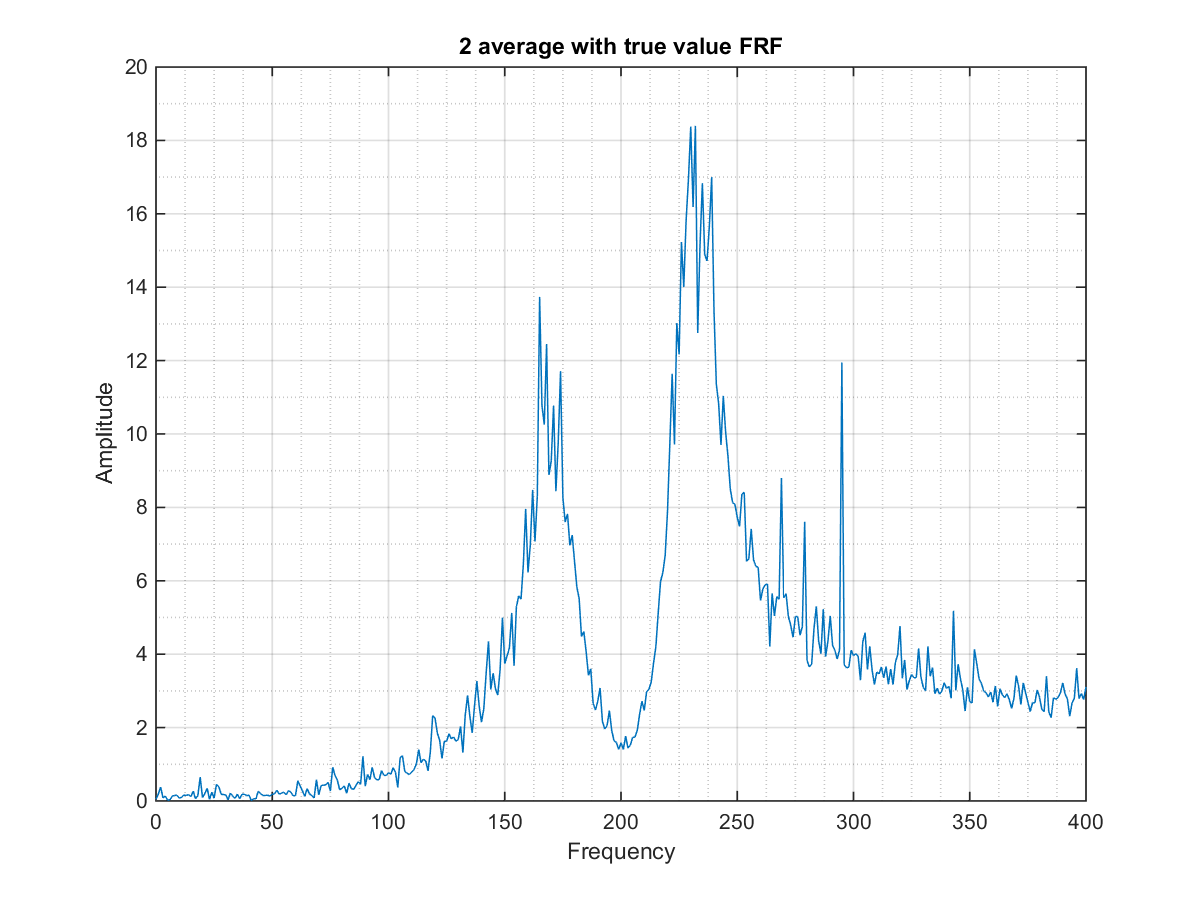
\includegraphics[scale=0.4]{fn4_VB1_1.png}
	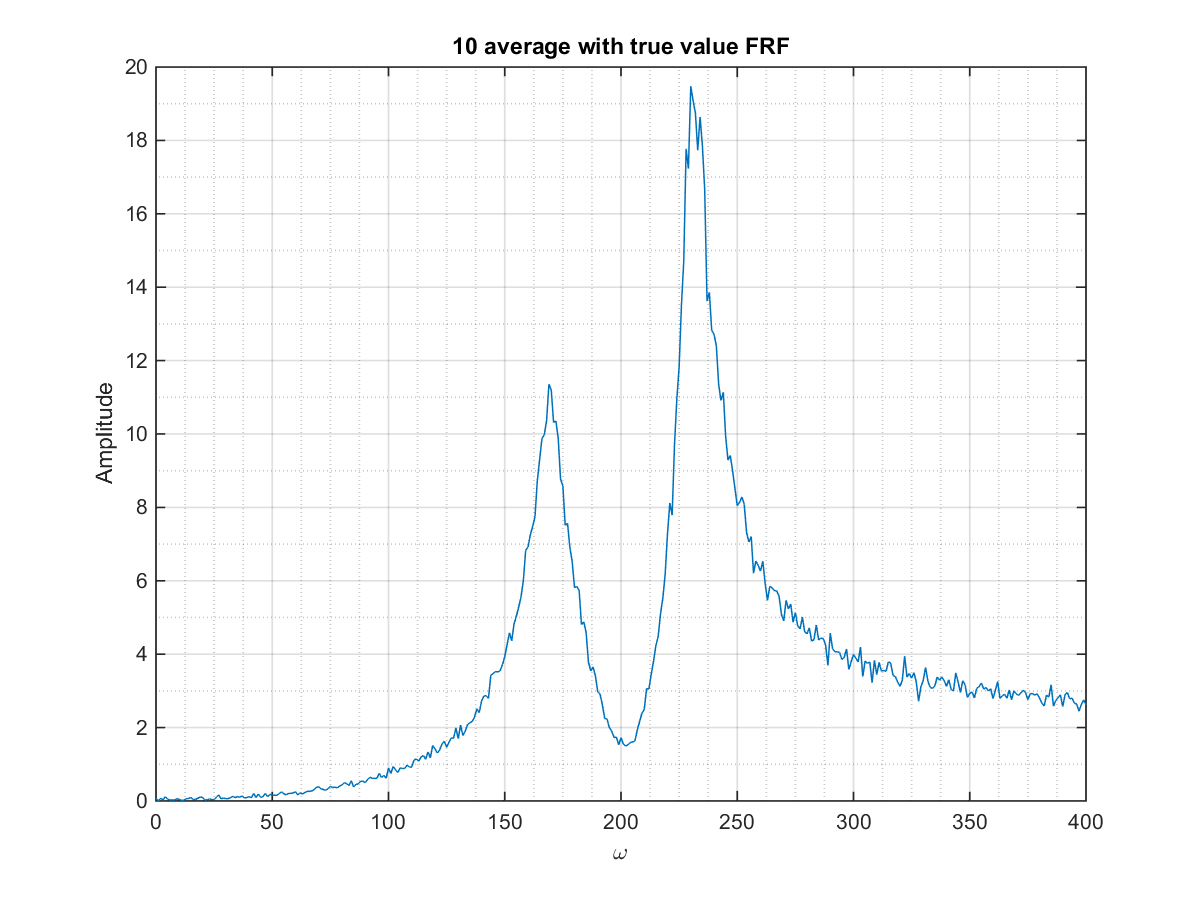
\includegraphics[scale=0.4]{fn4_VB1_2.png}
	\caption{FRF $H_c$ for 2 and 10 average with true FRF}
\end{figure}\\
2. The coherence $\gamma_{FX}^2$
\begin{figure}[htp]
	\centering
	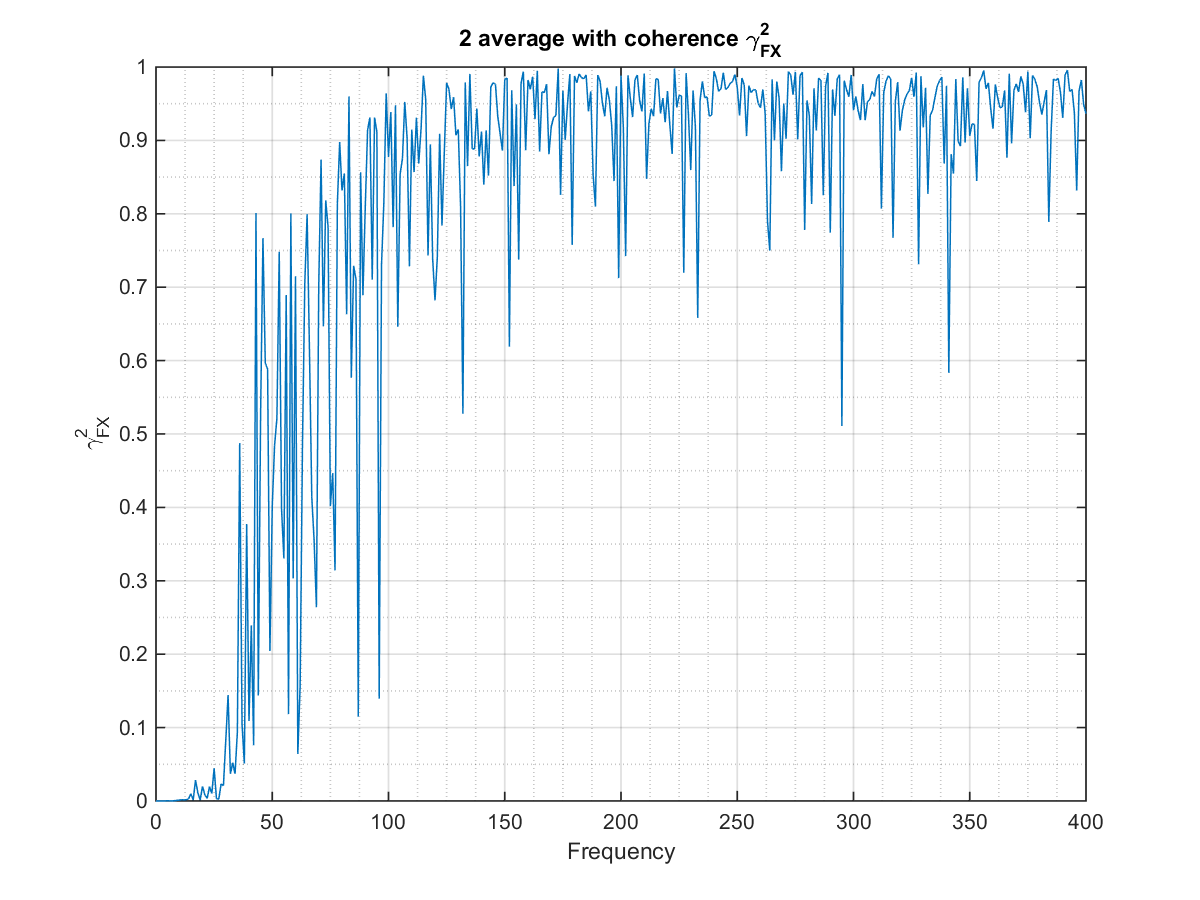
\includegraphics[scale=0.4]{fn4_VB2_1.png}
	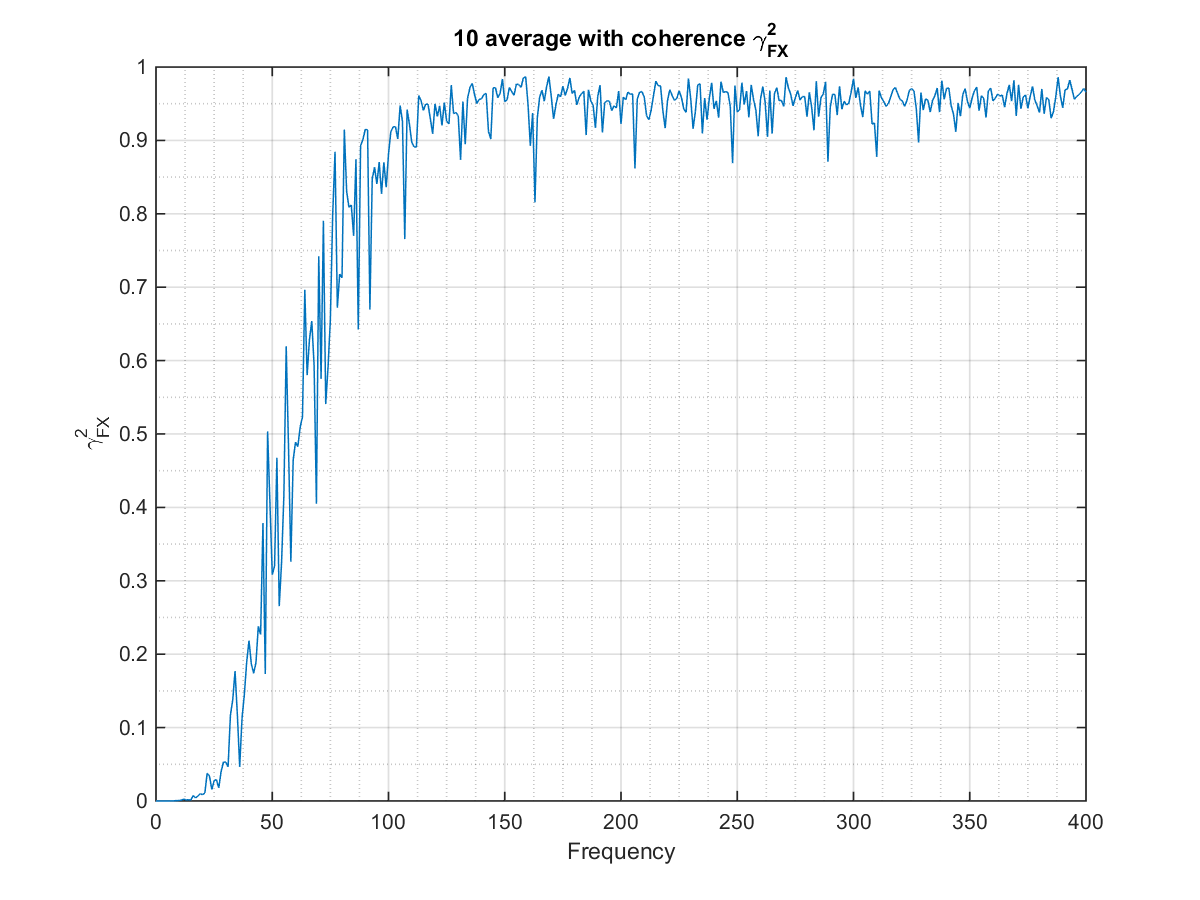
\includegraphics[scale=0.4]{fn4_VB2_2.png}
	\caption{Coherence $\gamma_{FX}^2$ for 2 and 10 average}
\end{figure}\\

\pagebreak

3. The single-sided spectral densities
\begin{figure}[htp]
	\centering
	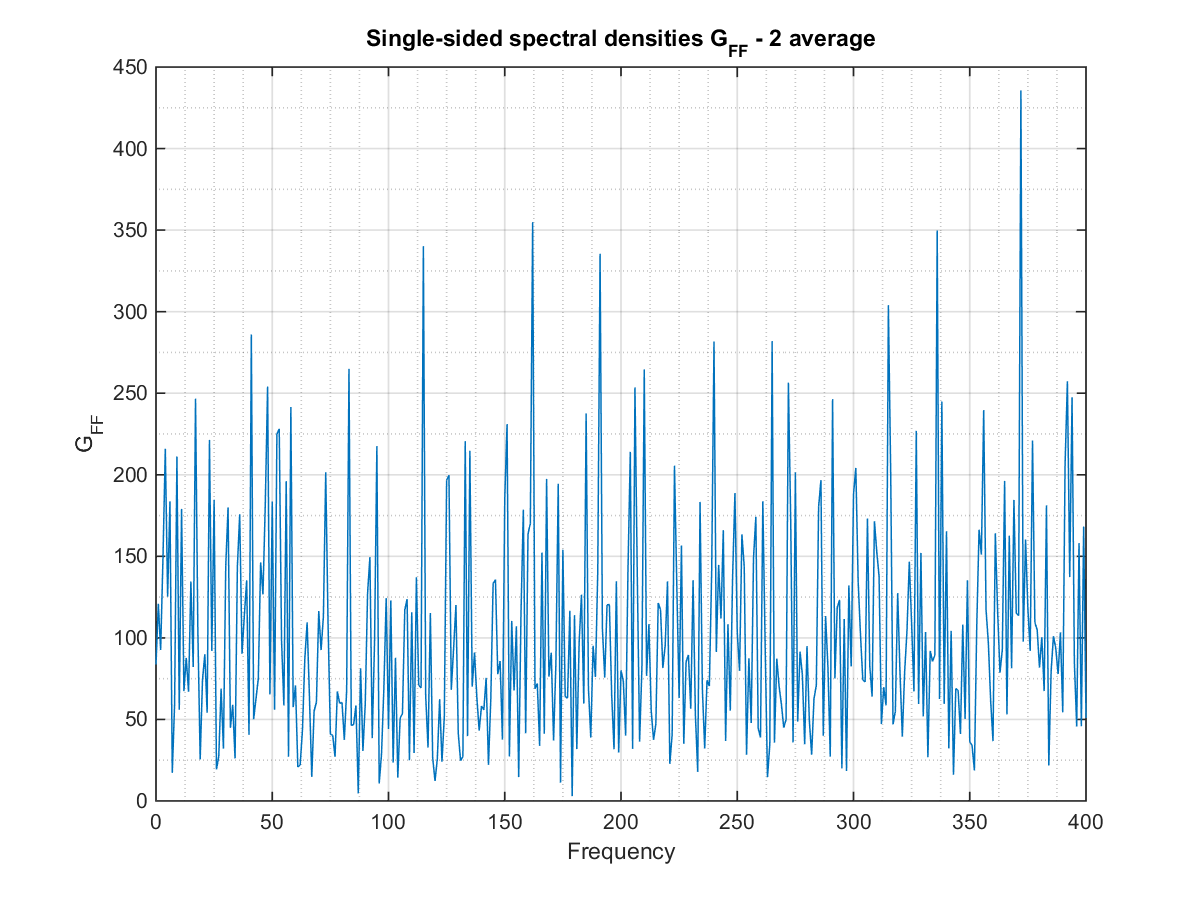
\includegraphics[scale=0.4]{fn4_VB3_1.png}
	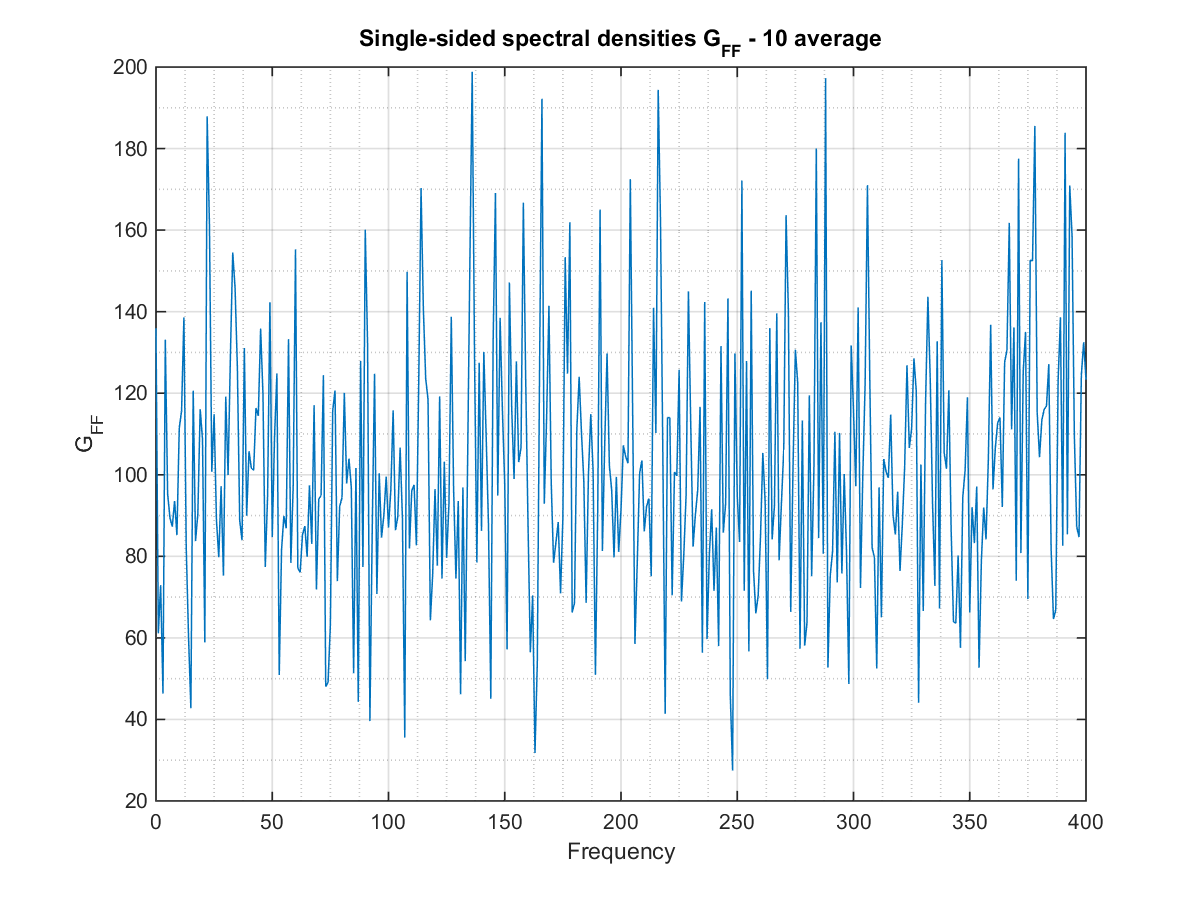
\includegraphics[scale=0.4]{fn4_VB3_3.png}
	\caption{The single-sided spectral $G_{FF}$ for 2 and 10 average}
\end{figure}
\begin{figure}[htp]
	\centering
	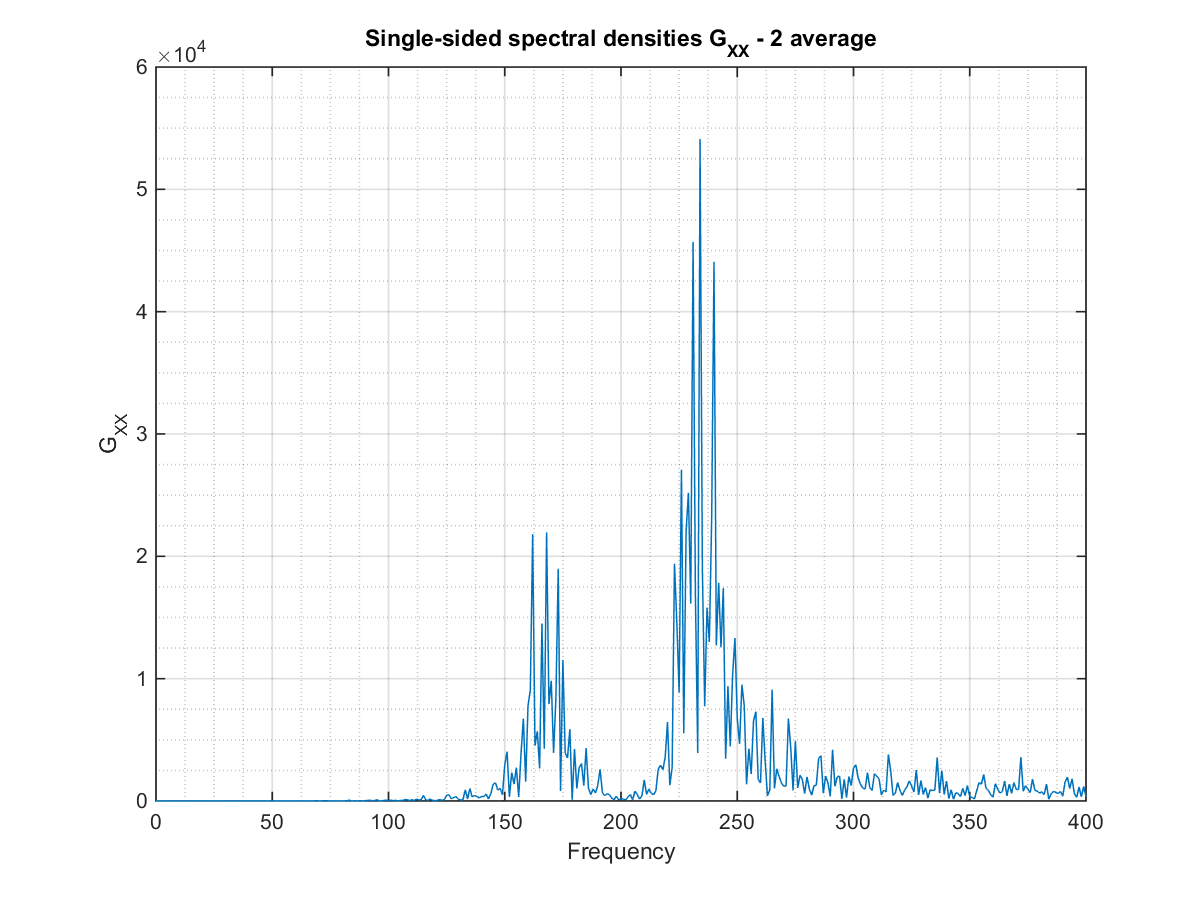
\includegraphics[scale=0.4]{fn4_VB3_2.png}
	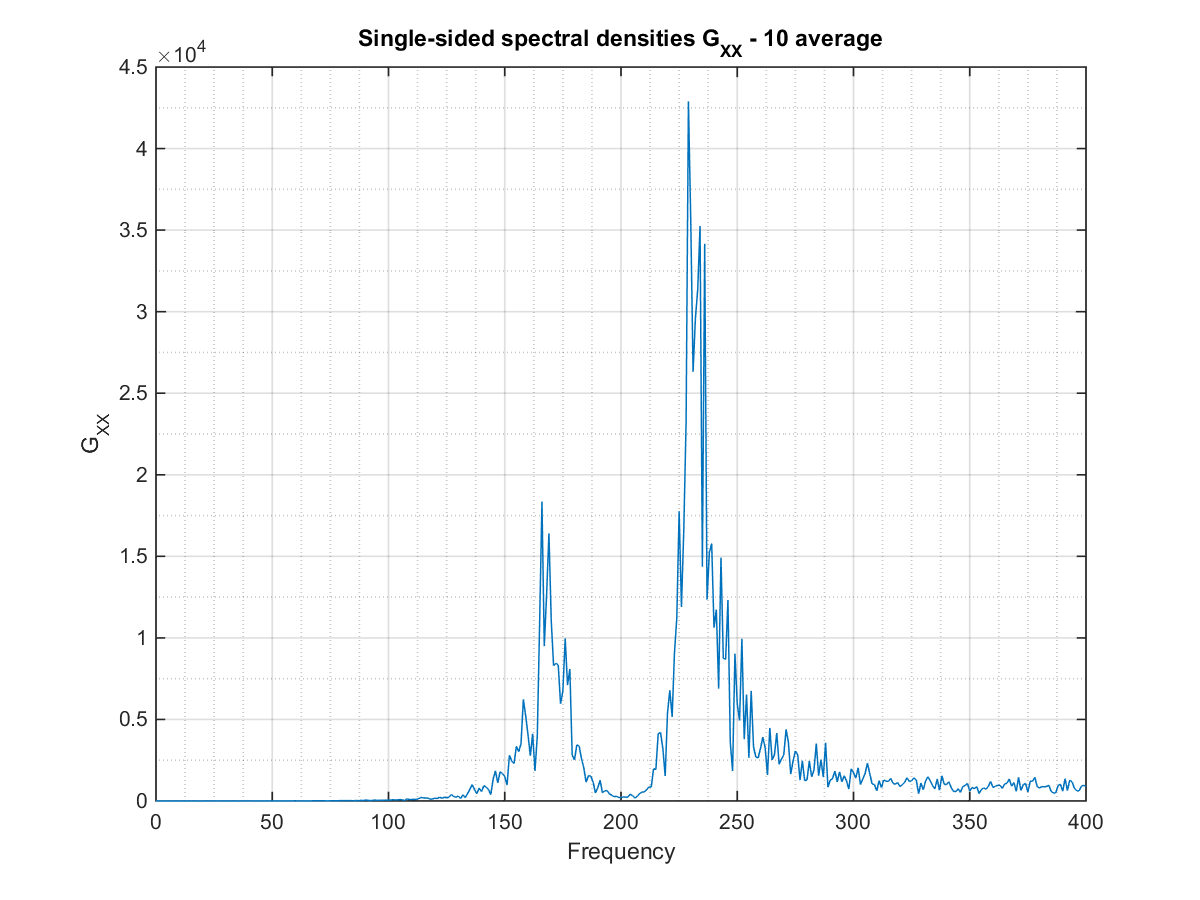
\includegraphics[scale=0.4]{fn4_VB3_4.png}
	\caption{The single-sided spectral $G_{XX}$ for 2 and 10 average}
\end{figure}\\
\pagebreak

4. Overlay the value of $H_c$ for 2 and 10 average on true value FRF we have:
\begin{figure}[htp]
	\centering
	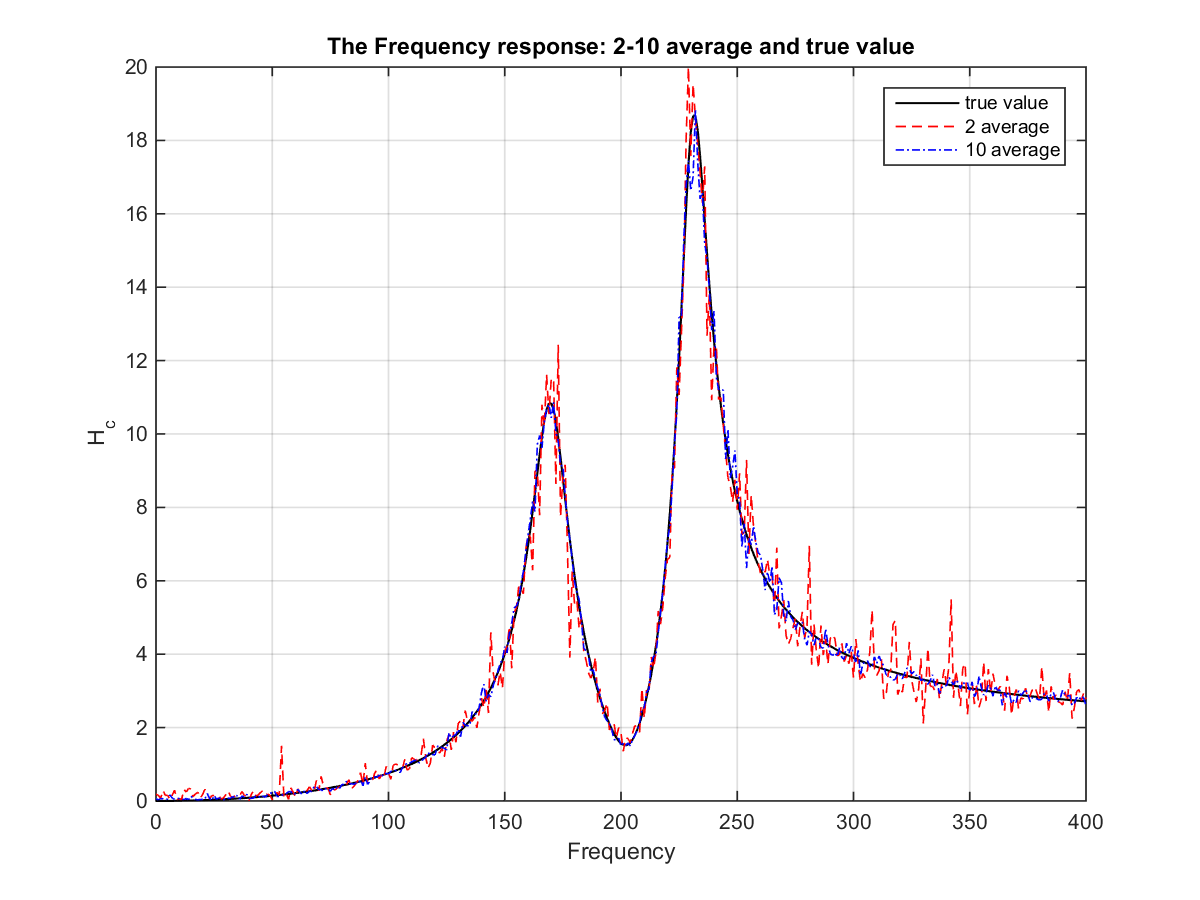
\includegraphics[scale=0.8]{fn4_VB4_1.png}
	\caption{The $H_c$ of true FRF and 2-10 average estimated}
\end{figure}\\
We see that in both estimated (with 2-average and 10-average), the mean of $H_c$ still very closed to the true value of FRF $\Rightarrow H_c$ is an unbiased estimator.

\end{document}